\PassOptionsToPackage{dvipsnames,svgnames,x11names}{xcolor}
\providecommand{\tightlist}{%
  \setlength{\itemsep}{0pt}\setlength{\parskip}{0pt}}
\documentclass[12pt]{article}
\usepackage[french]{babel}
\usepackage[utf8]{inputenc}
\usepackage{url}
\usepackage{array}
\usepackage{minted}
\usepackage{tabularx}
\usepackage{setspace}
\usepackage{abstract}
\usepackage{subfig}
\usepackage{listings}
\usepackage{amsmath}
\usepackage{graphicx}
\usepackage{iftex}
\usepackage{stmaryrd}
\usepackage[colorlinks]{hyperref}
\usepackage[top=2cm, bottom=2cm, left=2cm, right=2cm]{geometry}
\usepackage{titlesec}           % Pour changer la tailles ses sections/subsections...
\usepackage{algorithmic}        % Pour manipuler les algorithmes
\usepackage{algorithm}          % Pour manipuler les algorithmes
% \usepackage{algpseudocode}
\usepackage[absolute,overlay]{textpos} % Pour bouger les figures
\usepackage[nottoc]{tocbibind} %Includes "References" in the table of contents
\usepackage{listings}
\usepackage{xcolor}
\usepackage{fancyvrb}
\DefineVerbatimEnvironment{Highlighting}{Verbatim}{commandchars=\\\{\}}
\ifPDFTeX
  \usepackage[T1]{fontenc}
  \usepackage[utf8]{inputenc}
  \usepackage{textcomp} % provide euro and other symbols
\else % if luatex or xetex
  \usepackage{unicode-math} % this also loads fontspec
  \defaultfontfeatures{Scale=MatchLowercase}
  \defaultfontfeatures[\rmfamily]{Ligatures=TeX,Scale=1}
\fi
\usepackage{lmodern}
\ifPDFTeX\else
  % xetex/luatex font selection
  \setmainfont[]{Palatino}
  \setsansfont[]{Helvetica}
  \setmonofont[]{Menlo}
\fi
\allowdisplaybreaks
\colorlet{punct}{red!60!black}
\definecolor{background}{HTML}{EEEEEE}
\definecolor{delim}{RGB}{20,105,176}
\colorlet{numb}{magenta!60!black}
\lstdefinelanguage{minizinc}{
    morekeywords={
        constraint,int,
        maximize, solve, satisfy 
        var,
    },
    sensitive=true, % are the keywords case sensitive
    morecomment=[l][\em\color{ForestGreen}]{\%},
    %morecomment=[s]{/*}{*/},
    morestring=[b]",
}
\lstdefinelanguage{JavaScript}{
  keywords={typeof, new, true, false, catch, function, return, null, catch, switch, var, if, in, while, do, else, case, break},
  keywordstyle=\color{blue}\bfseries,
  ndkeywords={class, export, boolean, throw, implements, import, this},
  ndkeywordstyle=\color{darkgray}\bfseries,
  identifierstyle=\color{black},
  sensitive=false,
  comment=[l]{//},
  morecomment=[s]{/*}{*/},
  commentstyle=\color{purple}\ttfamily,
  stringstyle=\color{red}\ttfamily,
  morestring=[b]',
  morestring=[b]"
}

\lstset{
   language=JavaScript,
   backgroundcolor=\color{lightgray},
   extendedchars=true,
   basicstyle=\footnotesize\ttfamily,
   showstringspaces=false,
   showspaces=false,
   numbers=left,
   numberstyle=\footnotesize,
   numbersep=9pt,
   tabsize=2,
   breaklines=true,
   showtabs=false,
   captionpos=b
}
\lstset{
 basicstyle=\normalfont\ttfamily,
 language=caml,
 columns=[c]fixed,
 keywordstyle=\bfseries,
 upquote=true,
 commentstyle=,
 breaklines=true,
 frame=lines,
     numbers=left,
    numberstyle=\scriptsize,
    backgroundcolor=\color{background},
 showstringspaces=false,
 stringstyle=\color{blue},
 literate={'"'}{\textquotesingle "\textquotesingle}3
}
\lstdefinelanguage{json}{
    basicstyle=\normalfont\ttfamily,
    numbers=left,
    numberstyle=\scriptsize,
    stepnumber=1,
    numbersep=8pt,
    showstringspaces=false,
    breaklines=true,
    frame=lines,
    backgroundcolor=\color{background},
    literate=
     *{0}{{{\color{numb}0}}}{1}
      {1}{{{\color{numb}1}}}{1}
      {2}{{{\color{numb}2}}}{1}
      {3}{{{\color{numb}3}}}{1}
      {4}{{{\color{numb}4}}}{1}
      {5}{{{\color{numb}5}}}{1}
      {6}{{{\color{numb}6}}}{1}
      {7}{{{\color{numb}7}}}{1}
      {8}{{{\color{numb}8}}}{1}
      {9}{{{\color{numb}9}}}{1}
      {:}{{{\color{punct}{:}}}}{1}
      {,}{{{\color{punct}{,}}}}{1}
      {\{}{{{\color{delim}{\{}}}}{1}
      {\}}{{{\color{delim}{\}}}}}{1}
      {[}{{{\color{delim}{[}}}}{1}
      {]}{{{\color{delim}{]}}}}{1},
}
% Changement des commandes pour les algorithmes 
\renewcommand{\algorithmicrequire}{\textbf{Entrée(s)}}
\renewcommand{\algorithmicensure}{\textbf{Sortie(s)}}
\renewcommand{\algorithmicdo}{\textbf{faire}}
\renewcommand{\algorithmicforall}{\textbf{pour tout}}
\renewcommand{\algorithmicendfor}{\textbf{fin du pour}}
\renewcommand{\algorithmicif}{\textbf{si}}
\renewcommand{\algorithmicendif}{\textbf{fin du si}}
\renewcommand{\algorithmicthen}{\textbf{alors}}
\renewcommand{\algorithmicelse}{\textbf{sinon}}
\renewcommand{\algorithmicelsif}{\textbf{sinon si}}
\renewcommand{\algorithmiccomment}{\STATE //}
\setcounter{secnumdepth}{5}
\hypersetup{
    colorlinks,
    citecolor=black,
    filecolor=black,
    linkcolor=black,
    urlcolor=black
}

%pour ecrire chiffres romains
\makeatletter
\newcommand*{\rom}[1]{\expandafter\@slowromancap\romannumeral #1@}
\makeatother

\begin{document}

%régler l'espacement entre les lignes
\newcommand{\HRule}{\rule{\linewidth}{0.5mm}}


\titleformat{\chapter}{\bfseries\Large}{\arabic{chapter}.~}{0pt}{}   % Changer la taille des sections dans tout le document
\begin{titlepage}
      \center % Center everything on the page


      %----------------------------------------------------------------------------------------
      %	HEADING SECTIONS
      %----------------------------------------------------------------------------------------

      \textsc{\LARGE Sorbonne Université}\\[1.5cm] % Name of your university/college
      \textsc{\Large Rapport Final}\\[0.5cm] % Major heading such as course name
      {\large 19 Mai 2023}\\ % Date, change the \today to a set date if you want to be precise
      %\textsc{\large Minor Heading}\\[0.5cm] % Minor heading such as course title


      %----------------------------------------------------------------------------------------
      %	TITLE SECTION
      %----------------------------------------------------------------------------------------

      \vspace{2cm}
      \HRule \\[0.4cm]
      { \huge \bfseries Projet STL: \\ - \\ Interface pour Autobill}\\[0.7cm] % Title of your document
      \HRule \\[1cm]


      %----------------------------------------------------------------------------------------
      %	AUTHOR SECTION
      %----------------------------------------------------------------------------------------

      \begin{minipage}{0.4\textwidth}
            \begin{flushleft} \large
                  \emph{Auteurs:}\\
                  Brahima \textsc{Dibassi} \\
                  Zeid \textsc{Fazazi}\\
                  Yukai \textsc{Luo}
                  \vspace{2.5cm}
            \end{flushleft}
      \end{minipage}
      ~
      \begin{minipage}{0.55\textwidth}
            \begin{flushright} \large
                  \emph{Encadrants:} \\
                  Hector \textsc{Suzanne}\\ % Supervisor's Name
                  Emmanuel \textsc{Chailloux}\\ % Supervisor's Name
                  \textsc{}

                  \vspace{2.5cm}
            \end{flushright}
      \end{minipage}\\[1cm]

      % If you don't want a supervisor, uncomment the two lines below and remove the section above
      %\Large \emph{Author:}\\
      %John \textsc{Smith}\\[3cm] % Your name

      %----------------------------------------------------------------------------------------
      %	DATE SECTION
      %----------------------------------------------------------------------------------------


      %----------------------------------------------------------------------------------------
      %	LOGO SECTION
      %----------------------------------------------------------------------------------------

      
\includegraphics[scale=0.6]{Figures/Logo.png}\\[1cm] % Include a department/university logo - this will require the graphicx package

      %----------------------------------------------------------------------------------------

      \vfill % Fill the rest of the page with whitespace

\end{titlepage}
\newpage

{
      \hypersetup{linkcolor=}
      \setcounter{tocdepth}{3}
      \tableofcontents
}
\newpage

\section{Contexte du projet}\label{contexte-du-projet}
Dans le cadre de sa thèse sur l'analyse statique de consommation
mémoire d'un programme, notre tuteur de projet, Hector Suzanne, membre de l'équipe APR du laboratoire LIP6, a développé \textbf{\cite{autobill}}. \\
L'analyse statique est un ensemble de méthodes formelles permettant de
mesurer et détecter automatiquement des comportements ou des erreurs dans un
programme en examinant son code source. Parmi les usages les plus courants
de l'analyse statique, il y a le débogage pour identifier des erreurs
syntaxiques (fautes de frappe) ou l'usage de variables non déclarées ou
non-initialisées. D'autres outils emploient des heuristiques et des règles pour répondre à des problématiques d'optimisation de code ou de fiabilité/sécurité. Ces analyseurs statiques sont conçus dans le but d'améliorer la maintenabilité du code. \\
Autobill s'intéresse particulièrement à l'occupation mémoire d'un programme. Historiquement,
ce sujet de recherche a été plusieurs fois abordé dans divers travaux scientifiques, parmi eux, ceux de Jan Hoffmann et Steffen Jost sur l'analyse de consommation de ressources automatisé AARA
\cite{Hoffmann} (\emph{Automatic Amortized
      Resource Analysis}).\\
Cette technique suit un ensemble de règles d'inférence : chaque trait du langage analysé est annoté par ses bornes mémoire et on peut déduire la consommation mémoire que ce trait va engendrer. Pour déterminer ces bornes, l'AARA s'aide de l'analyse amortie par la méthode du potentiel. En effet, l'analyse amortie exploite la structure séquentielle des opérations sur des structures de données dynamiques pour calculer le coût total de cette séquence. Avec la méthode du potentiel, on attribue un potentiel aux structures de données manipulées, ce qui va affecter le coût que va avoir une opération sur cette structure. L’application de ces règles d'inférence sur l'ensemble des expressions du programme fournit une estimation correcte de ses bornes mémoires.
\begin{figure*}[!b]
      \centering
      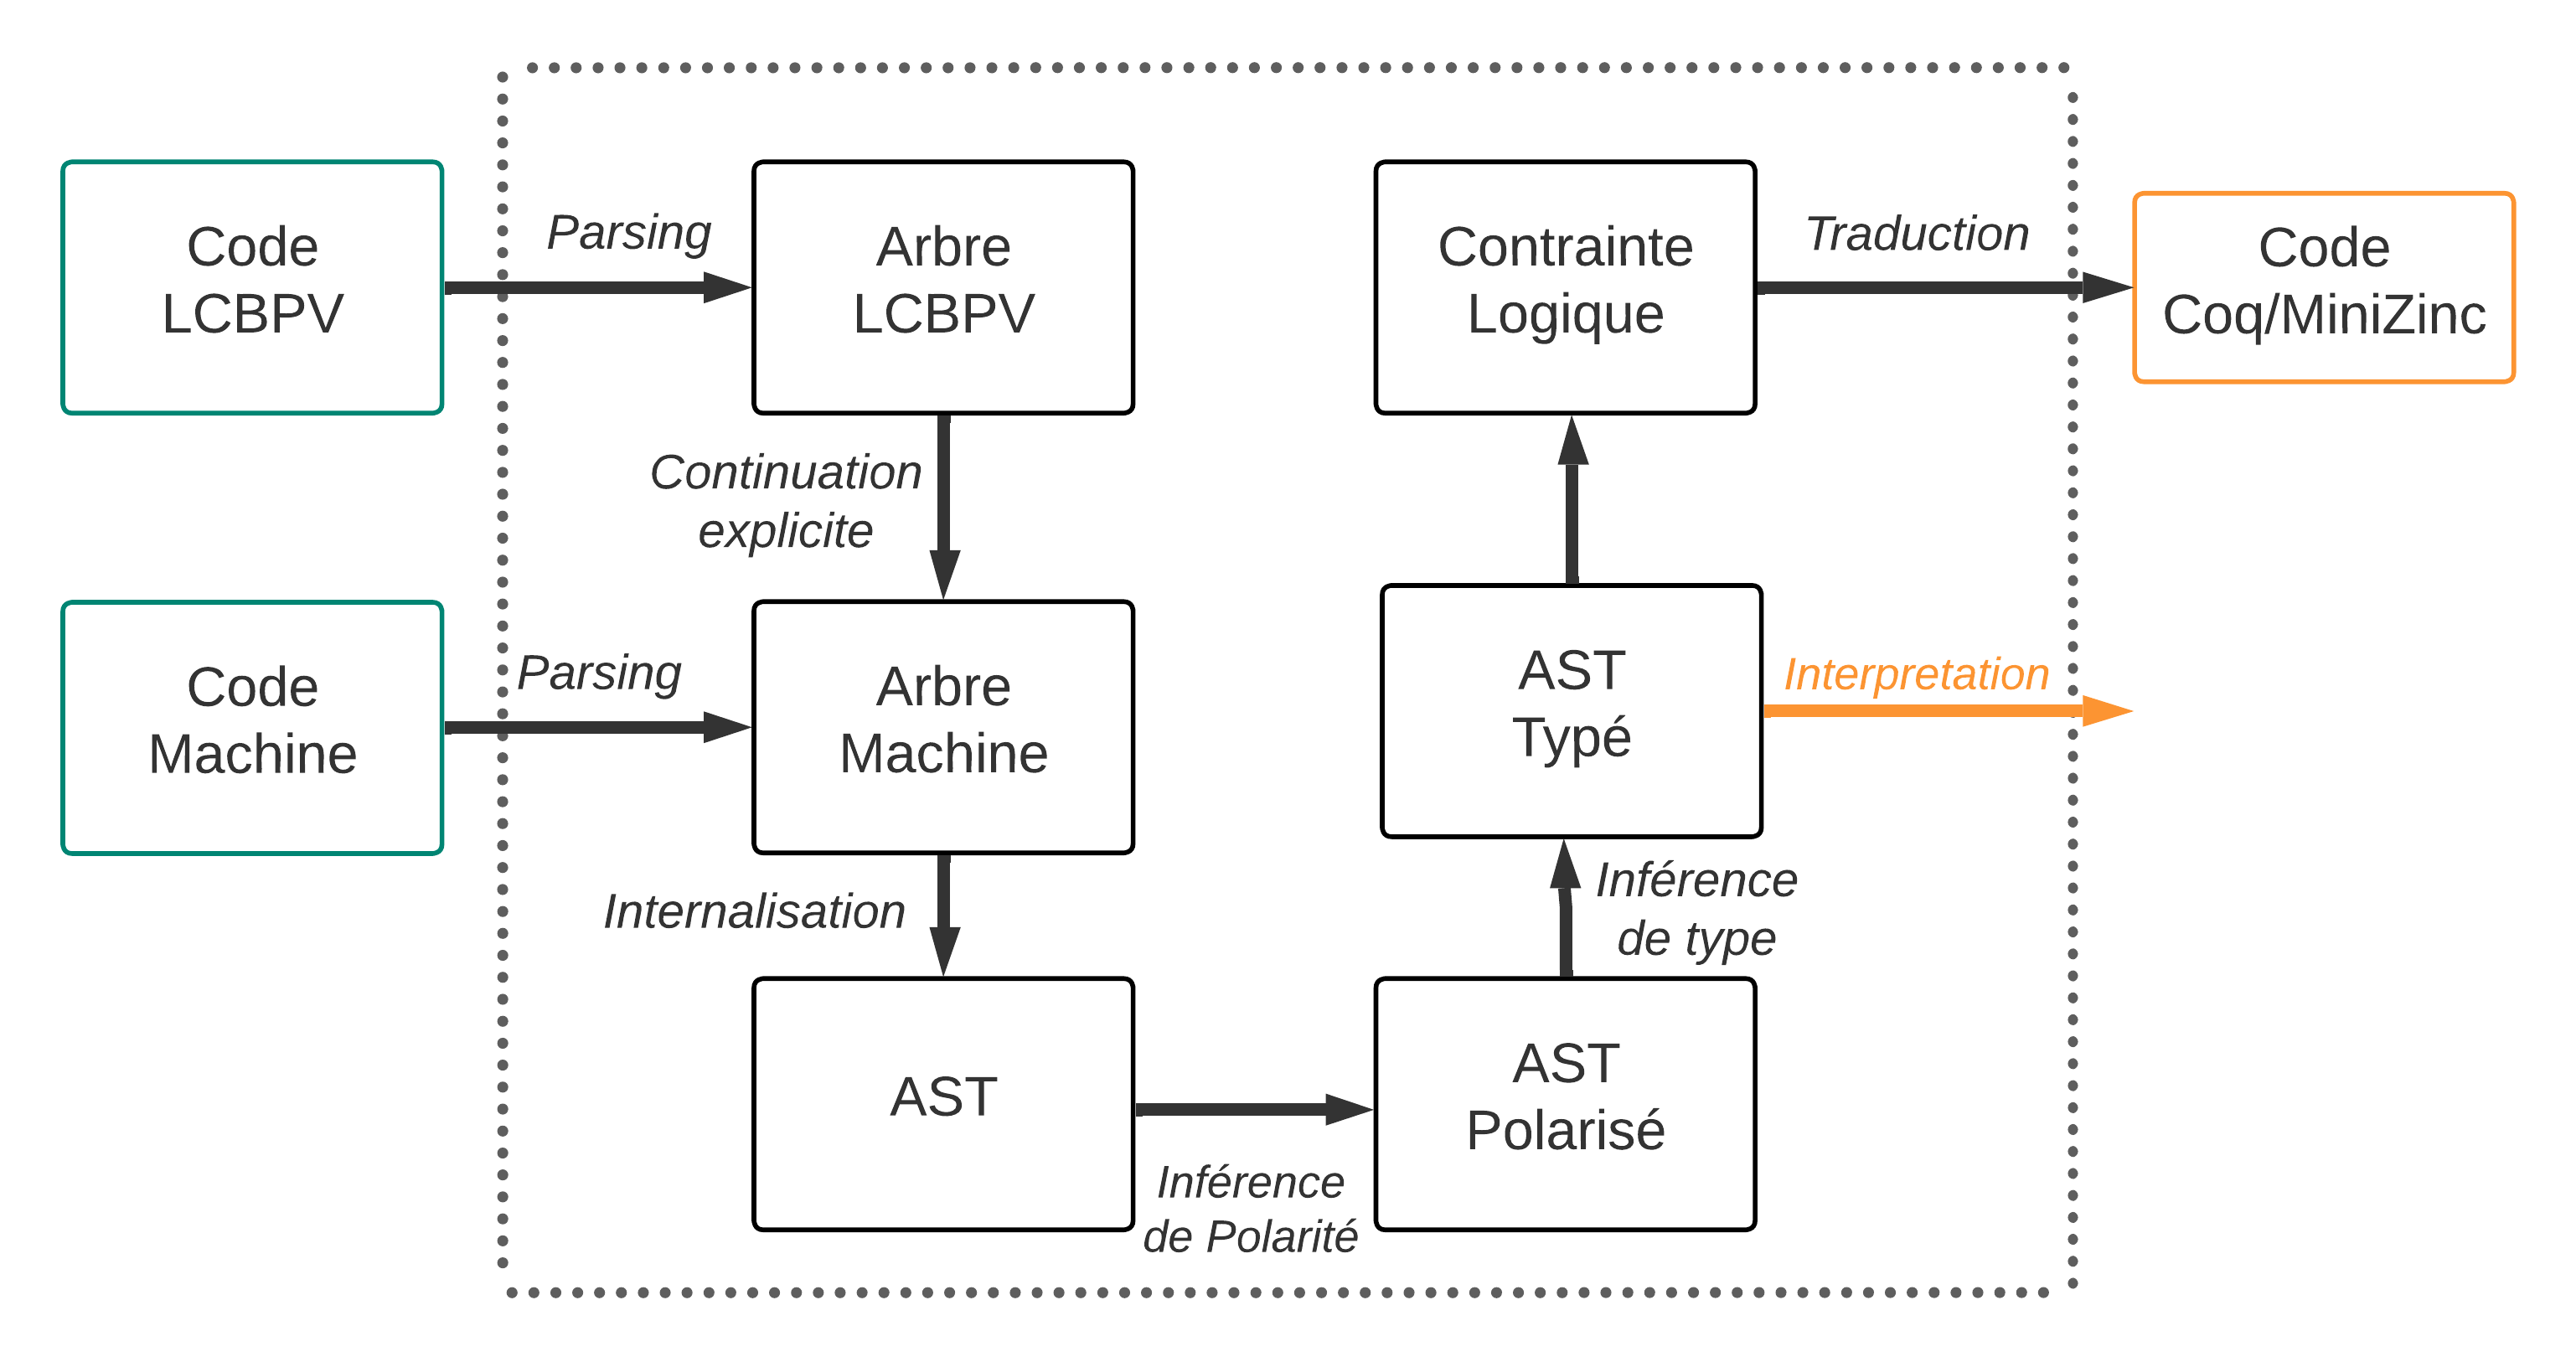
\includegraphics[scale=0.55]{Figures/Schema_Autobill.png}
      \caption{Représentation simplifiée d'Autobill\label{fig1}}
\end{figure*}

\pagebreak
\subsection{Historique et définitions}\label{historique-et-définitions}
Des langages de programmation expérimentaux ont vu le jour et ont implémenté cette analyse. On peut citer comme exemple Resource Aware ML \cite{RAML}, un langage fonctionnel à la ML créé par Jan Hoffmann, Klaus Aehlig et Martin Hofmann.

\hypertarget{quest-ce-quautobill}{%
      \subsection{Qu'est-ce qu'Autobill ?}\label{quest-ce-quautobill}}

La proposition d'Hector Suzanne avec Autobill se différencie par un
niveau d'analyse plus précis sur les fermetures et les arguments
fonctionnels d'un programme par rapport à RAML. D'abord, parmi les entrées possibles
illustrées sur la gauche de la Figure \ref{fig1}, Autobill ne supporte
uniquement que des programmes écrits soit en modèle machine propre à
Autobill, soit en \textbf{Call-By-Push-Value} (CBPV)
\cite{Levy}, avec ou sans continuation
explicite. \\

Call-By-Push-Value est un langage qui utilise un paradigme déjà éprouvé,
décrit dans la thèse de Paul Blain Lévy
\cite{Levy}. Dans CBPV, toutes les valeurs et fonctions sont stockées dans une pile. Lorsqu'une fonction est appelée, ses arguments sont placés sur la pile. Ce mécanisme permet de suivre de manière explicite la fonction appelée/terminée. Aussi,
le langage permet d'exprimer clairement les stratégies d'évaluation utilisées dans le code source : soit en \textbf{\textit{call-by-value}}, en évaluant les arguments avant de lancer l'opération, soit en \textbf{\textit{call-by-name}}, en évaluant les arguments uniquement lorsqu’ils seront effectivement utilisés dans la fonction appelée. Ainsi, on fixe quand les évaluations se déroulent afin de mieux prédire la consommation de mémoire à chaque
étape du programme. Ces traits font de CBPV un langage de choix à analyser pour Autobill. \\

L'entrée est donc imposée. Ainsi, pour étendre l'usage d'Autobill à un
autre langage de programmation, un travail de traduction de ce langage
donné vers CBPV doit avoir lieu. Cela implique donc de comprendre le
langage que l'on compile, notamment les stratégies d'évaluations
implicites mises en œuvre, et de l'adapter aux caractéristiques uniques
de CBPV citées plus haut. \\

À partir d'une entrée en CBPV, Autobill traduit le programme en un code
machine avec continuations explicites, exprimant explicitement les
contraintes de taille qui s'appliquent sur l'entrée. Il l'internalise,
c'est-à-dire construit l'arbre syntaxique abstrait (AST) de ce
programme. Ensuite, Autobill infère dans l'AST le typage de ses
expressions ainsi que leurs polarités, pour démarquer les calculs et les
valeurs dans l'AST. Enfin, en sortie, on remarque dans la Figure
\ref{fig1} la possibilité de tirer une interprétation du programme, mais
surtout de récupérer les contraintes dans un format MiniZinc
\cite{minizinc} ou Coq
\cite{coq}. Ce sont des outils qui permettent, à l'aide d'un langage dédié, d'exprimer
explicitement des contraintes logiques. Autobill s'en sert pour décrire
les bornes mémoires nécessaires au fonctionnement d'un programme. On
peut alors traiter ces équations avec des solveurs, fournis aussi par
ces deux outils, pour prouver des propriétés de complexité temporelle ou
spatiale.

\newpage

\subsection{Objectifs du projet}\label{objectifs-du-projet}

Notre démarche se rapproche de celle de RAML
\cite{RAML} avec leur site officiel: offrir
une interface Homme-Machine accessible à tous et illustrant un sujet de
recherche en analyse statique.

Le sujet de notre projet STL va donc être de soutenir l'effort de
développement en proposant une interface sur le Web permettant la libre
manipulation de l'outil Autobill par des utilisateurs à travers un
environnement de développement sur navigateur. On souhaite
aussi faciliter l'utilisation de l'outil avec un langage fonctionnel pur
en entrée plus accessible, un \textbf{MiniML}. Cela nous contraint donc
à adapter cette nouvelle entrée pour qu'elle soit compatible avec
Autobill. Enfin, on se chargera également de traiter les différentes sorties
standards et d'erreurs d'Autobill, notamment les expressions de
contraintes, afin de les passer à des solveurs externes, en tirer des
preuves de complexité et les afficher directement sur le client Web.

Par rapport à la chaîne d'instructions d'Autobill et à la Figure
\ref{fig1}, on se place donc en amont du code LCBPV en entrée et après
la sortie en code MiniZinc/Coq.

Notre charge de travail doit se diviser en plusieurs tâches principales:

\begin{itemize}
      \item
            L'implémentation du langage MiniML et sa traduction vers CBPV
      \item
            La mise en place d'une interface Web
      \item
            La mise en relation entre l'interface Web et la machine Autobill
      \item
            Le traitement des contraintes d'Autobill par un solveur externe
      \item
            Les tests de performances et comparaisons avec les solutions
            existantes
\end{itemize}

\begin{figure}
      \centering
      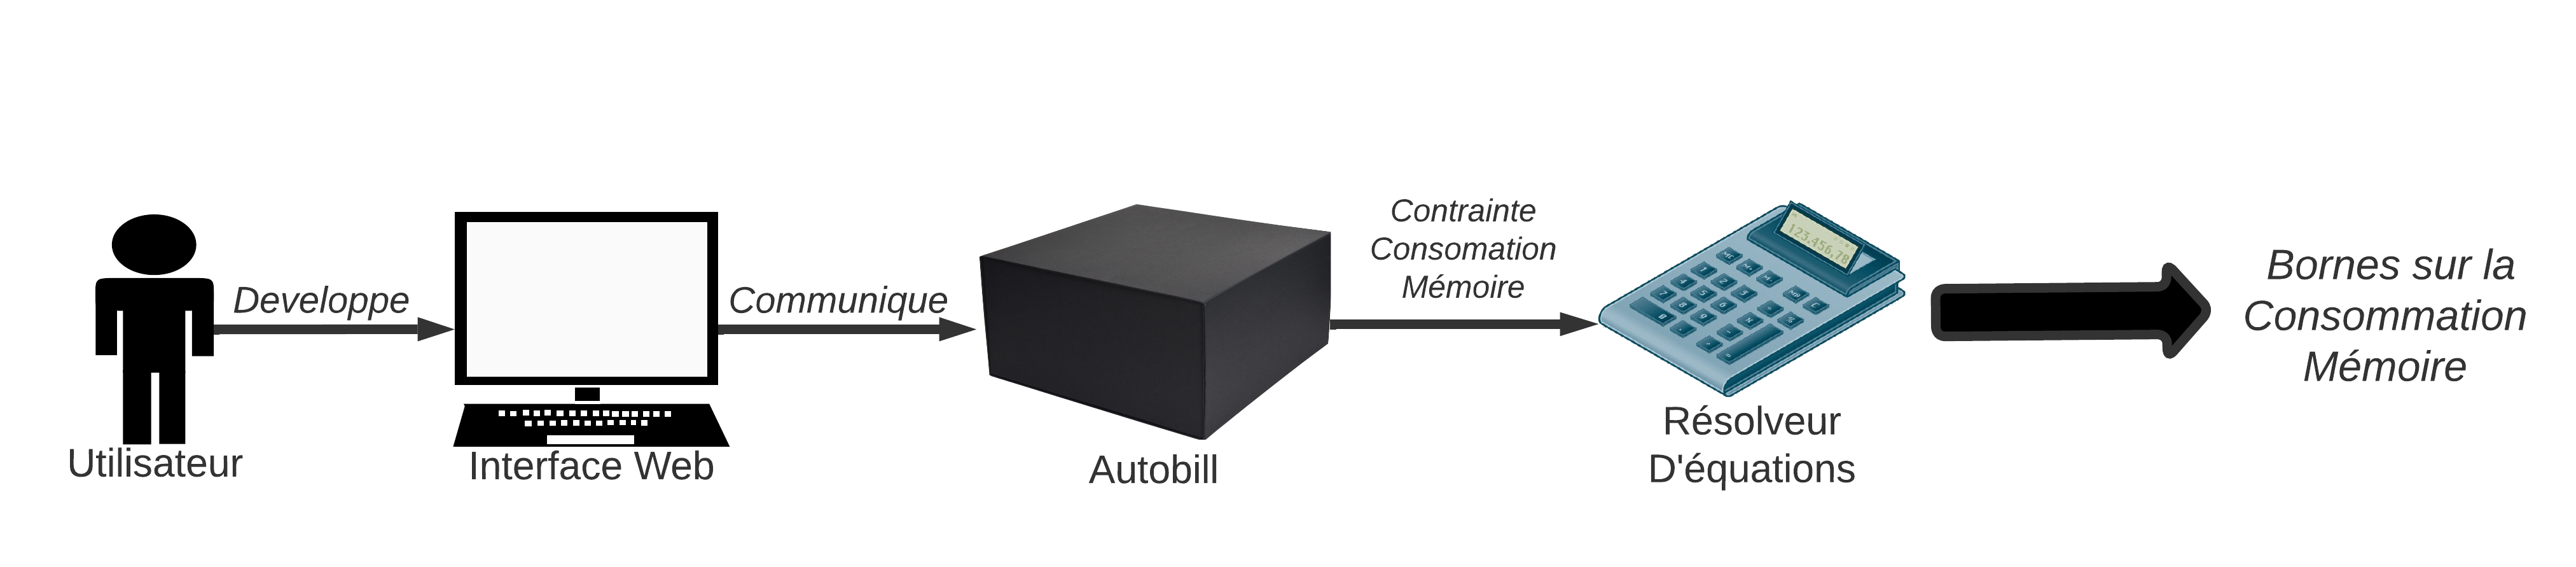
\includegraphics[scale=0.5]{Figures/DiagrammeHautNiveauPSTL.png}
      \caption{Représentation du système cible}
\end{figure}

\subsection{Processus de conception}\label{processus-de-conception}

Lors de la conception de l'interface, les contraintes étaient multiples.
La première était l'interopérabilité des technologies du projet. En
effet \textbf{Autobill} étant développé en \textbf{OCaml}, il était
nécessaire de trouver des moyens pour l'adapter à un environnement Web.
La seconde contrainte était qu'il fallait développer cette interface en simultané
avec \textbf{Autobill} et ajuster notre travail en fonction des besoins
courants de nos encadrants. Mais la plus importante d'entre elles était
le souhait de nos encadrants que l'application soit principalement côté
client afin de simplifier son déploiement.

Une fois ces contraintes établies, nous avons dû, tout au long de ce
projet, effectuer des choix, que ce soit en matière de design ou de
technologies. Nous tenons donc à travers ce rapport à mettre en lumière
ces décisions, tout en décrivant le travail qu'elles ont engendré.

\newpage

\hypertarget{interface-web}{%
      \section{Interface web}\label{interface-web}}

Dans l'optique de ne pas se restreindre dans l'utilisation d'outils
notamment au niveau du solveur de contraintes, on s'est orienté
vers deux structures de projets différentes et indépendantes: l'une
fonctionnant avec un client unique, la seconde avec un serveur dédié et
un client qui expose ce serveur.

L'avantage réside dans le fait que, lors du développement, si un nouvel
outil est amené à être utilisé mais ne dispose pas de compatibilité sur
navigateur Web, alors le serveur peut répondre à ce problème. C'est
aussi un sujet de comparaison intéressant à présenter par la suite, que
ce soit au niveau des performances que du déploiement de ces solutions.

De cette démarche, il en résulte un code source d'environ 800 lignes,
client et serveur compris, faisant tourner notre IDE en ligne dans un
état fonctionnel.

\subsection{Client}

Une première approche tout client a été mise œuvre dès le début du
projet. Celle-ci permettait de garantir une facilité dans le déploiement
en ligne de notre solution. Cette partie se concentra sur la présentation de
notre client Web, de l'implémentation des fonctionnalités importantes et des problèmes rencontrés ainsi que leurs résolutions.

\subsubsection{Interopérabilité Web-Ocaml}\

Autobill est un projet entièrement codé en Ocaml, un langage de programmation multi paradigme compilé, et notre projet STL impose un environnement sur navigateur Web, fonctionnant exclusivement avec son langage de script Javascript. Avant de commencer tout codage, il est nécessaire de passer en revue l'état de l'art autour de la compilation et d'exécution de programmes Ocaml sur le Web. De ces recherches vont découler  des choix de conception qui vont nous impacter tout le long du semestre. \\

D'abord, il y'avait la piste des compilateurs vers WebAssembly. WebAssembly est un standard du W3C (World Wide Consortium) qui regroupe un bytecode (.wasm) et un environnement d'exécution compatible avec les navigateurs modernes Javascript. Le bytecode étant une représentation très bas niveau de l'exécutable, l'idée principale étant de compiler un langage de programmation plus haut niveau, comme C/C++, scheme,.. vers bytecode. Ce bytecode est par la suite compilé par l'environnement d'exécution dans le langage machine de l'hôte. Tant que le support d'un langage de programmation est garanti par un compilateur WebAssembly, il est possible de programmer des applications web complètes dans le langage de son choix ou réinvestir des programmes codés dans ces langages dans une application codée avec des technologies Web. \\
Pour le cas d'Ocaml, cette possibilité est offerte grâce au post-processeur Wasicaml\cite{wasicaml} : il offre un binaire qui prend en entrée un bytecode Ocaml et un fichier .wasm de destination pour traduire chaque instruction dans son équivalent en WebAssembly. Ainsi, on pourrait générer nos fichiers .wasm à partir des binaires d'Autobill et de notre compilateur MiniML, les intégrer à notre application Web et les appeler avec Javascript en leur fournissant les options nécessaires. Cette solution demande néanmoins une dépendance à un projet encore en phase expérimentale, avec certains traits d'Ocaml non intégrés (notamment certaines fonctions du module Unix).\\
\begin{figure}
      \begin{lstlisting}
$ ocamlc -o hello hello.ml
$ wasicaml -o hello_wasm hello
\end{lstlisting}
      \caption{Chaîne d'instructions pour générer le bytecode WebAssembly}
\end{figure}

La seconde piste émise par nos tuteurs de projet était l'utilisation de compilateurs Ocaml vers Javascript. La présentation du projet nous a notamment pointé vers Js\_of\_Ocaml \cite{js_of_ocaml}. C'est une librairie contenant, entre autres, un compilateur qui transpile du bytecode OCaml en Javascript et propose une grande variété de primitives et de types pour manipuler des éléments Javascript depuis OCaml. L'API de Js\_of\_OCaml est suffisamment fournie pour développer entièrement des applications web complètes et fonctionnelles. On profite alors de l'expérience développeur offerte par Ocaml avec son style de programmation fonctionnelle en y intégrant les traits nécessaires pour construire des pages Web dynamiques.\\

Il est aussi possible de l'utiliser en coopération avec une base de code Javascript déjà rédigée grâce à la fonctionnalité d'export offerte par Js\_of\_Ocaml. En effet, on pourrait avoir dans un objet Javascript plusieurs méthodes correspondant chacune à un mode d'exécution différent d'Autobill. Chaque méthode prend en entrée le code MiniML à traiter et réalise les transformations nécessaires pour générer la sortie demandée (voir Figure \ref{fig4}). On peut aussi tirer profit des exceptions d'Ocaml et de la capture des sorties d'erreurs offerte par Js\_of\_Ocaml pour rediriger les messages d'erreurs et les afficher à l'utilisateur. Une fois l'objet exporté et le fichier Ocaml compilé vers Javascript, n'importe quel fichier Javascript du projet pourra ensuite importer l'objet et accéder aux méthodes définies précédemment. On garde ainsi une liberté sur le choix de technologies pour construire notre application.\\

\begin{figure*}[!b]
      \begin{lstlisting}[language=caml]
Js.export
    "ml"
    (object%js
       method translate code =
         let stderr_buff = Buffer.create 100 in
         Sys_js.set_channel_flusher stderr (Buffer.add_string stderr_buff);
         let lexbuf = Lexing.from_string ~with_positions:true (Js.to_string code) in
         let res = string_of_lcbpv_cst (translate_ML_to_LCBPV lexbuf)
         object%js
           val resultat = Js.string res
           val erreur = Js.string (Buffer.contents stderr_buff)
         end
    end)
\end{lstlisting}
      \caption{Création et exportation d'un objet Javascript avec une méthode de traduction de MiniML vers CBPV \label{fig4}}
\end{figure*}
Enfin, une dernière piste suggérée a été l'utilisation de langages de programmation camélien compilables vers Javascript, comme ReasonML\cite{reasonml} ou Rescript\cite{rescript}. En effet, ce sont tous deux des langages qui ont émergé d'Ocaml et permettent de créer dans un paradigme fonctionnel des applications web complexes. Ils profitent d'une syntaxe ML, d'outils et d'un support communautaire intéressant, faisant des deux langages des alternatives intéressantes pour le Web. Néanmoins, notre objectif principal est la manipulation de la librairie d'Autobill ainsi que celle de MiniML depuis le Web. La compatibilité avec les librairies en Ocaml n'est cependant pas garantie dans le contexte d'une compilation vers Javascript. \\

Notre groupe a donc opté pour un choix de conception assez flexible afin de nous adapter aux situations que l'on pourrait rencontrer dans le projet. Le client fonctionnera conjointement grâce à une partie Ocaml servie à l'aide de Js\_of\_Ocaml et une partie en Javascript, plus précisément en React.js\cite{react}, pour assurer les fonctionnalités propres à notre IDE.

\subsubsection{L'éditeur de code}\

L'idée initiale était de proposer une interface de développement intégrée sur le Web. Celle-ci devait proposer les outils nécessaires pour réaliser les trois tâches suivantes : analyser, écrire et déboguer du code. Pour répondre à ces besoins, plusieurs composants essentiels vont devoir fonctionner ensemble pour fournir l'expérience d'un IDE classique :
\begin{itemize}
      \item Un éditeur de code pratique et adapté à l'écriture de code dans notre langage MiniML.
      \item Un menu de navigation entre les programmes proposés par l'application ou créés par l'utilisateur
      \item Un menu de sélection entre différentes configurations d'analyses
      \item Une sortie standard et d'erreur pour afficher le retour de l'analyse d'Autobill \\
\end{itemize}

La question de l'éditeur de code s'est rapidement posée pour nous. En effet, c'est sur ce composant que va être concentrée l'expérience de l'application et nous avions la volonté de nous rapprocher au plus d'une prise en main similaire aux IDE modernes (Visual Studio Code, Eclipse, IntelliJ...). L'idée d'utiliser un simple champ de texte agrandi n'était donc pas envisageable. \\

En premier lieu, l'effort de développement a été mis dans la construction \textit{from Scratch} d'un éditeur de code. Cela a permis de fixer clairement les exigences et les fonctionnalités que nous attendions d'un éditeur de code moderne. Déjà, il devait proposer une expérience d'écriture correcte avec toutes les manipulations usuelles et attendues : le comptage des lignes, la recherche et le remplacement rapide d'une suite de caractères (Ctrl+F), le \textit{linting} d'erreurs... Enfin, il y a le support du langage d'écriture des programmes. Par cela, il est question notamment de coloration syntaxique pour isoler les mots-clés et symboles réservés du langage mais aussi de l'autocomplétion basique.  \\

\begin{figure}
      \centering
      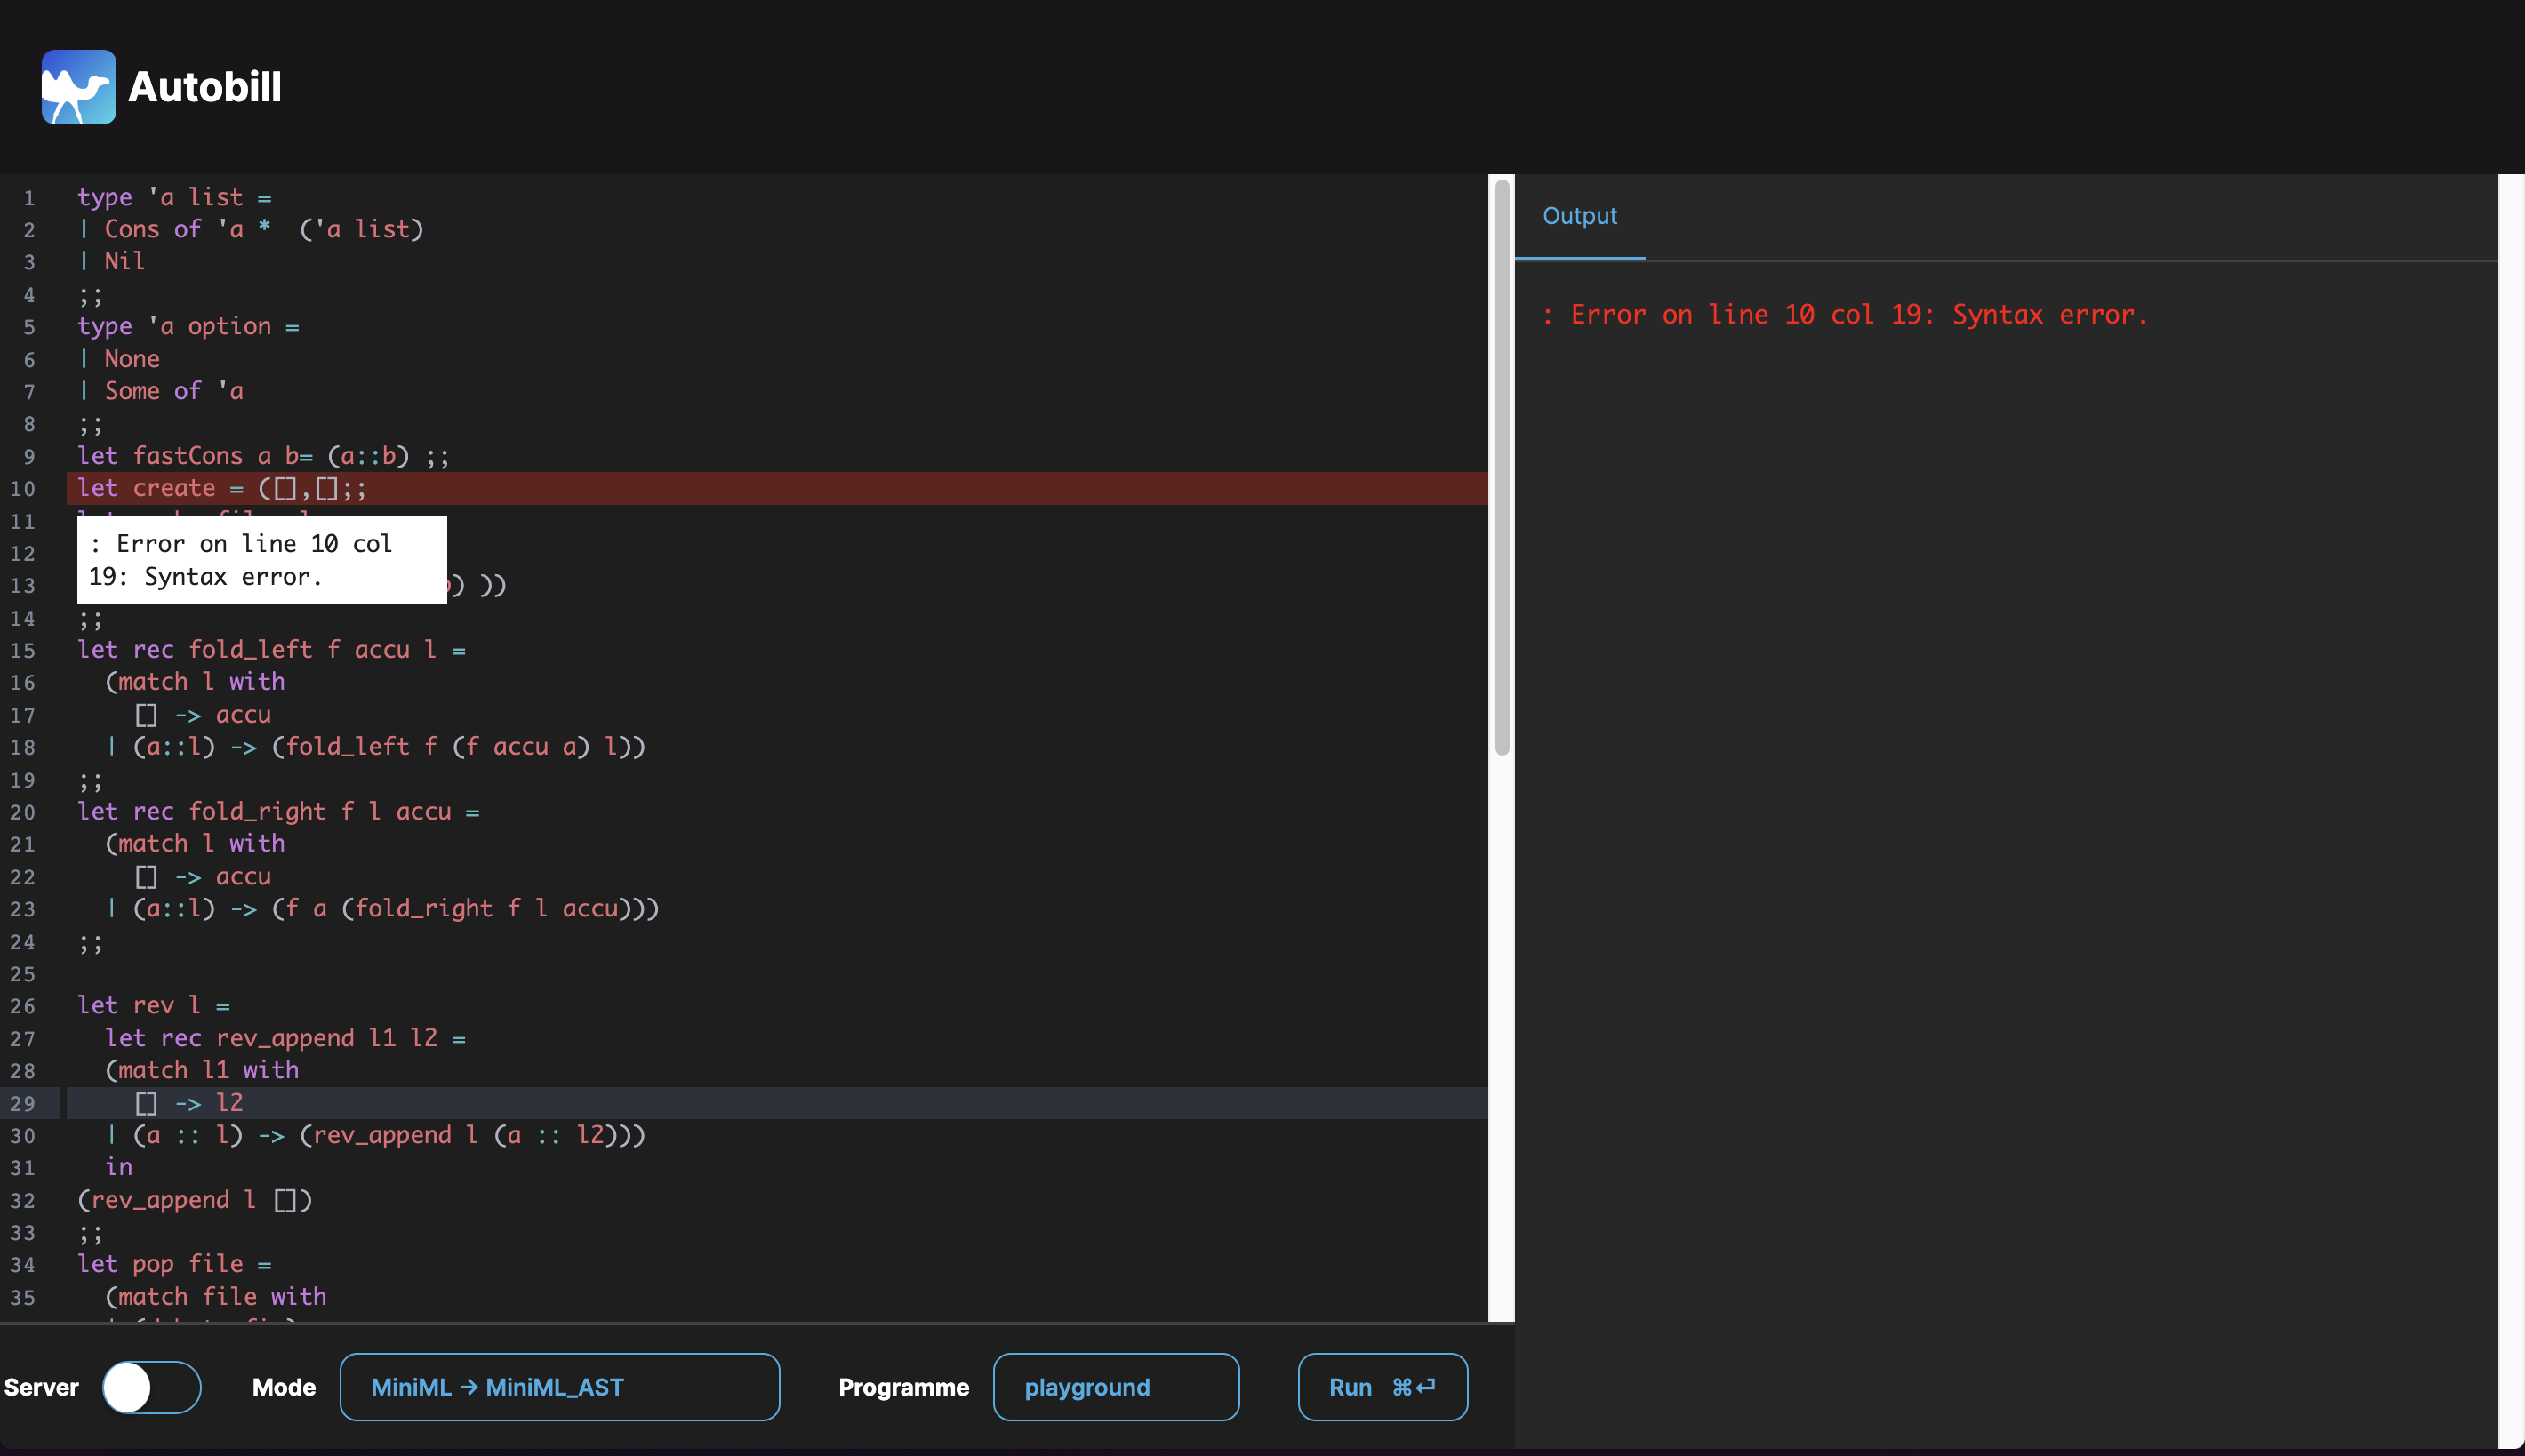
\includegraphics[scale=0.36]{Figures/screen.png}
      \caption{Interface pour Autobill, dans le scénario d'une erreur\label{fig5}}
\end{figure}
L'examen de nos besoins nous a donc contraints à repousser l'idée d'une création d'un éditeur en partant de zéro.
Délivrer les fonctionnalités citées plus haut tout en assurant la stabilité de la solution serait complexe et concentrerait beaucoup d'efforts sur ce composant, au détriment de chantiers clés comme le MiniML. C'est un élément de l'application d'autant plus important qu'il ne doit pas être négligé et demande à lui seul l'effort et le temps nécessaires à un projet universitaire pour être réalisé. Nous nous sommes donc tournés vers des librairies et solutions déjà existantes afin de les intégrer dans notre projet. \\

Parmi les librairies disponibles, nous avons choisi CodeMirror\cite{codemirror}. C'est un éditeur de code pour navigateur Web, disponible en libre de droits, qui peut s'intégrer à n'importe quelle application Web. Ses fonctionnalités sont exhaustives et il offre de multiples choix de personnalisations pour l'adapter à un langage spécifique. Nativement, il y a le support intégré pour la syntaxe de langage à la ML comme Ocaml ou F\# : MiniML étant un substrat, on peut aisément créer notre fichier de configuration pour ne garder que les mots-clés essentiels de notre langage et Codemirror s'occupe du parsing du code et de la coloration de chaque caractère. \\

Enfin, le \textit{linting} est disponible et permet de dynamiquement surligner des lignes de l'éditeur. Comme illustré dans la Figure \ref{fig5}, on peut, à la volée, afficher directement les parties du programme concernées par une erreur de l'analyse. En effet, quand une méthode de Js\_of\_Ocaml est appelée et qu'une exception est levée durant l'exécution, sa sortie d'erreur peut être redirigée et retournée directement au client. Côté Ocaml, on peut alors formater la sortie d'erreur avec les données de l'exception : la ligne de début et de fin, le type d'erreur rencontrée, la phase de l'analyse durant laquelle l'exception a été levée... \\
\begin{figure}
      \centering
      \begin{lstlisting}[language=json,firstnumber=1]
{
    "loc": {
        "beginning": { "line": 10, "column": 19},
        "end": {"line": 10, "column": 21}
    },
    "info": "Error on line 10 col 19: Syntax error."
}
\end{lstlisting}
      \caption{Sortie d'erreur Ocaml parsée\label{fig6}}
\end{figure}

Côté Web, on peut parser la chaîne de caractères et récupérer le JSON parsé pour manipuler les informations sur l'erreur rencontrée (voir Figure \ref{fig6}). CodeMirror offre des fonctions permettant de manipuler l'état global de l'éditeur: son thème, son contenu, le langage de la coloration syntaxique, les options activées... On y retrouve surtout la liste des lignes qui composent l'éditeur. On peut alors leur affecter des changements de style pour les mettre en lumière ou faire apparaître une infobulle avec le message d'erreur si on passe la souris dessus... \\

On offre ainsi les outils nécessaires à l'utilisateur pour bien écrire et déboguer son code MiniML. Néanmoins, il faut encore compléter la \textit{pipeline} en traitant toutes les sorties possibles d'Autobill, notamment les équations sur les contraintes mémoires du programme analysée qu'il va falloir résoudre.

\subsubsection{La résolution de contraintes}\

Autobill exprime les contraintes mémoires qui s'appliquent à un programme dans des formats proches d'équations mathématiques. Il propose de type de sortie : une sous Coq et une sous MiniZinc. Nous nous concentrerons principalement sur MiniZinc dans cette partie, Coq n'étant pas encore totalement opérationnel et demandant des ressources qui dépassent le cadre du Master d'informatique. \\

MiniZinc est un langage permettant de décrire des problèmes de manière déclarative à l'aide de contraintes logiques. Il fournit des éléments de syntaxe et de notations très similaires à la programmation et aux mathématiques pour rédiger des modèles qui, lorsqu'ils seront passés à des compilateurs et des solveurs dédiés, vont répondre à des problématiques d'optimisation ou de satisfiabilité. Dans notre cas, on s'intéresse à l'optimisation : on veut déterminer les bornes mémoires minimum du programme passé à Autobill.
Néanmoins, on rencontre un problème similaire qu'avec Autobill : la librairie est codée en C++, langage compilé, incompatible avec l'environnement Web. Là encore, l'option de WebAssembly est envisageable avec un compilateur comme Emscripten \cite{emscripten} qui supporte la traduction de code C/C++ vers bytecode WebAssembly. Ici, la librairie core de MiniZinc est beaucoup plus fournie et ne contient pas un point d'entrée direct explicite, comme avec le binaire d'Autobill. La compilation devient alors une tâche plus compliquée et la manipulation sûre de l'outil n'est pas non plus garantie par la suite. \\

Le support via une librairie Javascript qui utilise elle-même le bytecode WebAssembly est possible. Elle offre une interface entre le développeur et le logiciel MiniZinc via un ensemble d'objets et méthodes qui facilitent les interactions avec l'outil. Comme montré dans la Figure \ref{fig8}, quelques lignes suffisent pour créer son modèle et lancer les tâches de résolution, tout cela nativement dans la machine de l'utilisateur. Cette passerelle permise avec cette API nous permet de faire tourner le moteur de résolution de contraintes directement sur le navigateur et d'afficher les bornes mémoires nécessaires au programme dans l'interface. \\

Celle-ci prend la forme d'une équation polynomiale qui décrit la complexité spatiale du programme d'entrée. Dans l'exemple de la Figure \ref{fig8}, un unique coefficient non-nul est est attaché à x, ce qui suggère une complexité spatiale linéaire pour le programme depuis lequel les contraintes ont été dérivées. On remarque alors la limite dans l'analyse d'Autobill qui ne prend pas encore en compte des complexités logarithmiques ou quasi-linéaires. Des pistes sont encore en cours de développement : il y a notamment le passage des équations sur les contraintes mémoires au format Coq, mais aussi l'ajout de plusieurs raffinements / paramétrages dans la \textit{pipeline} entre MiniML et CBPV (présentée plus bas dans ce rapport) qui permettraient des dérivations de complexités plus précises. \\

\begin{figure}
      \centering
      \begin{lstlisting}[language=javascript]
        const model = new Model()
        model.addFile("playground.mzn", code)
        const solve = await model.solve({
          options: {
            solver: "gecode",
          },
        })
    \end{lstlisting}
      \caption{Création et résolution d'un modèle MiniZinc en Javascript}
      \includegraphics[scale=0.65]{Figures/Résolution.png}
      \caption{Affichage de la résolution sur l'interface\label{fig8}}
\end{figure}



\pagebreak

\hypertarget{serveur-client}{%
      \subsection{Serveur + client}\label{serveur-client}}

\subsubsection{Contexte}\

Dans le stade actuel d'Autobill, une architecture avec un client seul
peut répondre aux exigences du projet STL. Néanmoins, au fur et à mesure que le projet avançait, nous nous sommes rendu compte d'un problème. Autobill évolue constamment et rien ne garantit que ses itérations suivantes puissent
être supportées par notre solution. Par exemple, l'utilisation de la librairie core de Mini-Zinc peut échouer en mode client unique. En outre, on ne peut pas garantir que la génération de module Javascript par Js$\textunderscore$of$\textunderscore$Ocaml soit réussite dans le mode client-seulement.  Donc dans l'optique de rendre notre solution plus flexible et \emph{future proof}, une nouvelle version de notre interface, qui déporte les tâches complexes vers un serveur distant, a été développée. Parce que dans une architecture client-serveur, la librairie child$\textunderscore$process nous propose la solution. \\

La librairie child$\textunderscore$process est un module intégré à Node.js qui permet d'exécuter des processus enfants (child processes).  Il exploite les fonctionnalités du système d'exploitation sous-jacent pour créer et gérer les processus enfants et utilise des appels système spécifiques pour créer des processus enfants et établir une communication avec eux via des tubes. Il fournit une interface permettant de lancer d'autres programmes ou scripts à partir de notre application Node.js. Cela nous permet d'effectuer des tâches telles que l'exécution de commandes système, l'appel de programmes externes, le démarrage de processus en arrière-plan. Cependant, ce module child$\textunderscore$process est conçu pour interagir avec le système d'exploitation et exécuter des processus en dehors du navigateur. C’est une fonctionnalité spécifique à Node.js et ne peut pas être utilisé directement dans un environnement de développement front-end, qui s'exécute dans le navigateur. Cette fonctionnalité n'est donc pas disponible pour notre architecture client-seulement. Du coup, nous pensons qu'il soit vital de construire une architecture client-server pour assurer la stabilité et la flexibilité de notre travail.\\

On a souhaité aussi adapter le client pour qu'il opère dans ces deux
architectures différentes. Ainsi, dans notre environnement de
développement, on peut facilement faire la bascule entre un mode de
fonctionnement local/synchrone et un mode distant/asynchrone. \\

Comme on a mentionné dans la section 1, l'objectif de notre projet STL est de construire une pipeline du MiniML à la résolution de contrainte ( MiniML $\rightarrow$ LCBPV $\rightarrow$ Autobill $\rightarrow$ Équation $\rightarrow$ Résolution). Et nous voulons diviser notre architecture Client-Server en deux parties, la partie MiniML et la partie résolution de contraintes. Les services de la partie MiniML réalisent la partie MiniML $\rightarrow$ LCBPV $\rightarrow$ Autobill $\rightarrow$ Équation de la pipeline, puis les services de la partie résolution de contraintes réalisent la partie Équation $\rightarrow$ Résolution de la pipeline.\\

Pour cette architecture de client-serveur, on décide d’utiliser la méthode POST de HTTP, pour envoyer une requête qui contient le code écrit dans l'éditeur du code à serveur. Le serveur traite le code soit en utilisant le module généré par Js$\textunderscore$of$\textunderscore$Ocaml (Pour la partie MiniML, voir section 2.2.2), soit en utilisant la bibliothèque Childprocess, qui peut lancer l'exécution en passant les lignes de commande ( Pour la partie Résolution de contraintes, voir section 2.2.3 ). Après le traitement du code, le serveur renvoie le résultat au client.\\


\hypertarget{schuxe9ma-de-communication}{%
      \subsubsection{MiniML}\label{schuxe9ma-de-communication}}

\begin{figure}[!b]
      \centering
      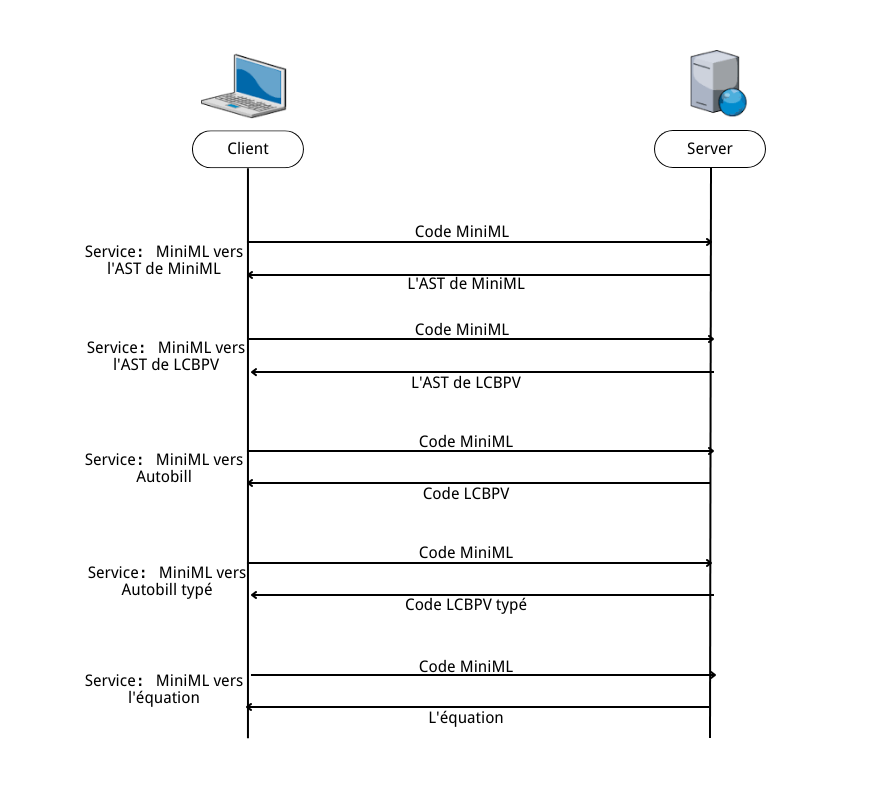
\includegraphics[scale=0.5]{Figures/CommunicationMiniML.png}
      \caption{Schéma de communication : MiniML\label{fig9}}
\end{figure}


Dans la partie MiniML, on utilise la méthode POST de HTTP, pour envoyer une requête qui contient le code écrit dans l'éditeur du code à serveur. Le serveur traite le code soit en utilisant le module généré par Js$\textunderscore$of$\textunderscore$Ocaml. Après le traitement du code, le serveur renvoie le résultat au client. Nous avons mis en place 5 services principaux en utilisant le protocole HTTP (voir Figure \ref{fig8}): '\emph{/MiniML/toMiniMLAST}', '\emph{/MiniML/toLCBPV}', \emph{'/MiniML/toAutobill'}, \emph{'/MiniML/toAutobillType'} et \emph{'/MiniML/toEquation'}. \\

Pour le service \emph{'/MiniML/toMiniMLAST'}, le client envoie le code du MiniML au serveur via une requête POST. Le serveur le transforme vers l'AST de MiniML et le renvoie au client. Et pour le service \emph{'/MiniML/toLCBPV'},le client envoie le code du MiniML au serveur via une requête POST. Le serveur le transforme vers l'AST de LCBPV et le renvoie au client. Ces deux services génèrent l'AST de MiniML et de LCBPV. Le côté client affiche l'AST sur le côté après avoir reçu la réponse HTTP. L'objectif principal de ces deux services est de valider les résultats du lexer, du parser et de la traduction, en nous aidant à finir l'écriture des ces trois parties.\\

Pour le service \emph{'/MiniML/toAutobill'}, le client envoie le code du MiniML au serveur via une requête POST. Le serveur le transforme vers sa version internalisé en code machine et le renvoie au client. Et pour le service \emph{'/MiniML/toAutobillType'}, le client envoie le code du MiniML au serveur via une requête POST. Le serveur le transforme vers le code machine d'Autobill typé et le renvoie au client. La côté client affiche le code LCBPV généré par le serveur après reçu la réponse HTTP. Ce deux services générent le code de LCBPV traduire par MiniML, cela fournit les sources d'entrée d'Autobill et complète la partie MiniML $\rightarrow$ LCBPV $\rightarrow$ Autobill dans le pipeline.\\

Pour le service \emph{'/MiniML/toEquation'}, le client envoie le code du MiniML au serveur via une requête POST. Le serveur le transforme vers l'équation résultant de l'analyse statique et le renvoie au client. Ce service permet de générer les équations de l'analyse statique, dans format de code MiniZinc, en utilisant le service correspondant dans Autobill. Ces équations seront utilisées pour obtenir les bornes de consommation de mémoire dans les services suivants, mentionnés dans la section 2.2.3. Ce service complète la partie MiniML $\rightarrow$ LCBPV $\rightarrow$ Autobill $\rightarrow$ Équation dans la pipeline. Mais ce service correspondant dans Autobill est encore en progrès, H.Suzanne est en train de l'améliorer pour obtenir le meilleur résultat. Donc finalement on ne peut pas encore obtenir les équations directement depuis le code MiniML.

\subsubsection{La résolution des contraintes}\
Pour la partie la résolution des contraintes, on utilise la méthode POST de HTTP, pour envoyer une requête qui contient le code écrit dans l'éditeur du code à serveur. Le serveur exécute le code et renvoie le résultat au client. Donc l'objectif de cette partie est l'exécution des équations en format MiniZinc généré par Autobill, et l'obtention des bornes de consommation de mémoire de programme. Pour exécuter le code MiniZinc, on a trouvé deux moyens. Le premier est d'utiliser la librairie de MiniZinc généré par bytecode WebAssembly comme mentionné dans la section 2.1.3. Et la deuxième manière utilise la librairie child$\textunderscore$process, qui nous permet d'effectuer l'exécution des programmes MiniZinc en passant les lignes de commande.\\

D'abord on écrit le code dans un fichier temporaire. Et on prépare une ligne de commande qui exécute un fichier MiniZinc en le passant à 'Gecode', un solveur externe de MiniZinc. Puis on utilise la méthode exec() qui permet d'exécuter notre commande dans un shell système et de récupérer la sortie dans un tampon. Elle prend en paramètre la commande à exécuter et une fonction de callback. La fonction de callback reçoit éventuellement une erreur, la sortie standard et la sortie d'erreur du processus. (voir Figure \ref{fig10}) Dans la partie résolution de contraintes, nous avons un service \emph{'/minizinc/gecode'} qui exécute le code MiniZinc (Voir Figure \ref{fig11}). Le client envoie le code de MiniZinc au serveur via une requête POST. Le serveur exécute le code, et renvoie le résultat au client.

\begin{figure}
      \centering
      \begin{lstlisting}[language=javascript]
    const fs = require('fs');
    const tmpFile = './temp.mzn';
    fs.writeFileSync(tmpFile, code);
    const cmd = `minizinc --solver Gecode ${tmpFile}`;
    exec(cmd, (error, stdout, stderr) => {
        fs.unlink('temp.mzn', (err) => {
            if (err) throw err;
        });
    }
\end{lstlisting}
      \caption{Exécution de code Minizinc\label{fig10}}
\end{figure}



\begin{figure}
      \centering
      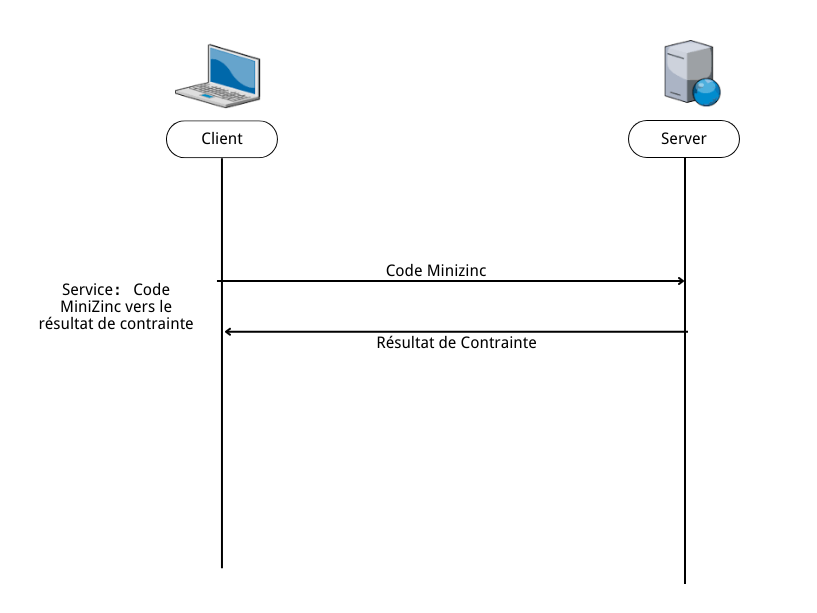
\includegraphics[scale=0.5]{Figures/CommunicationMiniZinc.png}
      \caption{Schéma de communication : MiniZinc\label{fig11}}
\end{figure}

\newpage
\hypertarget{miniml}{%
      \section{MiniML}\label{miniml}}

\hypertarget{description-de-miniml}{%
      \subsection{Description de MiniML}\label{description-de-miniml}}

\textbf{MiniML} émerge du choix de nos encadrants de créer un langage
fonctionnel simple et accessible pour les utilisateurs d'Autobill
servant d'abstraction à \textbf{CBPV}. Nous avons pris la décision de rendre la syntaxe MiniML parfaitement
compatible avec OCaml simplifiant les comparaisons avec d'autres outils utilisant \textbf{OCaml} en entrée.

Le développement de \textbf{MiniML} suivant les besoins de nos
encadrants, celui-ci est sans effets de bord.

\hypertarget{Caractéristiques-de-miniml}{%
      \subsection{Caractéristiques de MiniML}\label{Caractéristiques-de-miniml}}

Une fois les besoins de nos encadrants définis, nous avons pu définir les caractéristiques de \textbf{MiniML}.
Il s'agit d'un langage fonctionnel pur représentant uniquement la partie fonctionnelle d'OCaml.
Pour ce faire, nous avons premièrement mis en place en ensemble minimal permettant un $\lambda$-calcul simple et efficace.
\textbf{MiniML} permet donc comme toute implémentation du $\lambda$-calcul simple :
\begin{itemize}
      \item L'utilisation de variables
      \item L'application de fonctions
      \item La définition de fonctions
      \item La définition de fonctions récursives
\end{itemize}
Ensuite pour permettre une utilisation plus simple et plus proche de la famille ML, nous avons ajouté la notion de types tel que décrite dans le \textbf{Système F}\cite{SystemF}\cite{SystemF2}.\\
\textbf{MiniML} devient donc un $\lambda$-calcul typé de la famille ML grâce à l'ajout en autres des fonctionnalités suivantes :
\begin{itemize}
      \item La définition de types algébriques avec les types somme et produit et la possibilité de les imbriquer
      \item La définition de constructeurs de types algébriques
      \item La définition et l'utilisation de types polymorphes \footnote{Par manque de temps dû à quelques essais infructueux, nous n'avons pas pu implémenter les annotations de types rendent peut-être possible la création de problèmes de typage indécidables.}
      \item Des types de base : \textbf{entier}, \textbf{booléen}, \textbf{singleton}
            \footnote{On notera l'absence de certains types de base tel que les flottants. Ces derniers n'étant pas pris en charge à l'heure actuelle par \textbf{Autobill}.}
\end{itemize}
\hfill \break
Une fois les caractéristiques de \textbf{MiniML} définies, nous avons pu commencer à travailler sur la spécification de ce dernier, en commençant par la grammaire.
\hfill \break
\pagebreak

\hypertarget{grammaire}{%
      \subsection{Grammaire}\label{grammaire}}


\newcommand{\grammarRule}[1]{\; \textbf{<\textcolor{Blue}{#1}>} \;}
\newcommand{\grammarRuleUnSpaced}[1]{\textbf{<\textcolor{Blue}{#1}>}}
\newcommand{\nTime}[1]{\; #1\text{*} \;}
\newcommand{\nPlus}[1]{\; #1\text{+} \;}
\newcommand{\isToken}[1]{\; \textit{`\textcolor{Maroon}{#1}`} \;}
\newcommand{\isTokenLCBPV}[1]{\; \textit{`\textcolor{Green}{#1}`} \;}
\newcommand{\isRangeToken}[2]{\; \textit{`\textcolor{Maroon}{#1} - \textcolor{Maroon}{#2}`} \;}
\newcommand{\isExtentionML}[1]{ \textit{\textcolor{Orange}{#1}} \quad }

Voici la grammaire BNF du langage MiniML.\
Pour des raisons de lisibilité, tous les éléments de sucre syntaxiques ne seront pas détaillés ici.\
Les extensions non compatibles avec OCaml mais compatibles avec \textbf{Autobill} sont en \textcolor{Orange}{Orange}.

\hypertarget{Éléments Nommés}{%
      \subsubsection*{Éléments Nommés}\label{Éléments Nommés}}

On appelle éléments nommés, les identificateurs \grammarRule{Id} pour les variables, motifs et types, les identificateurs de constructeurs \grammarRule{ConstructeurId} et les variables de types \grammarRule{Vartype}

\begin{align*}
      \grammarRule{Id} ::= \quad             & \nPlus{[\isRangeToken{a}{z} \isRangeToken{A}{Z} \isRangeToken{0}{9} \isToken{\_}]} \\
      \grammarRule{ConstructeurId} ::= \quad & [\isRangeToken{A}{Z}] \grammarRule{Id}                                             \\
      \grammarRule{Vartype} ::= \quad        & \isToken{'}[\isRangeToken{a}{z}] \; \nTime{[\isRangeToken{0}{9}]}
\end{align*}

\hypertarget{programmes}{%
      \subsubsection*{Programmes}\label{programmes}}

On définit un programme \textbf{MiniML} comme une expression précédée de zéro ou plusieurs définitions néccessaires à son évaluation.
\begin{align*}
      \grammarRule{Prog} ::= \quad & |\quad \grammarRule{Expr}                                  \\
                                   & |\quad \grammarRule{Def}  \isToken{;;}  \grammarRule{Prog}
\end{align*}

\hypertarget{definitions}{%
      \subsubsection*{Définitions}\label{definitions}}

On définit au sein de la règle de grammaire \grammarRule{Def} deux constructions :
\begin{itemize}
      \tightlist
      \item
            Les définitions de \textbf{Variables Globales},
      \item
            Les définitions de \textbf{Types}.
\end{itemize}

\begin{align*}
      \grammarRule{Def} ::= \quad & |\quad \isToken{let} \grammarRule{Id} \isToken{=} \grammarRule{Expr}                                                  \\
                                  & |\quad \isToken{type} \nTime{\grammarRuleUnSpaced{Vartype}} \grammarRule{Id} \isToken{=} \grammarRule{NewContructors} \\
\end{align*}

\subsubsection*{Définitions de Constructeurs}\label{defConstruct grammar}
On définit au sein de la règle de grammaire \grammarRule{NewContructors} deux constructions :
\begin{itemize}
      \tightlist
      \item
            Les définitions de \textbf{Constructeurs Classiques} qui sont compatibles avec OCaml.
      \item
            Les définitions de \textbf{Constructeurs Equationnels} qui sont une extension spécifique pour \textbf{Autobill} incompatible avec OCaml permettant de définir des constructeurs de types algébriques avec des équations.
\end{itemize}
\begin{align*}
      \grammarRule{NewContructors} ::=   \quad & |\quad  \grammarRule{ConstructeurId} \isToken{of} \grammarRule{Type}                                            \\
                                               & |\quad  \grammarRule{NewContructors} \isToken{|} \grammarRule{NewContructors}                                   \\
      \isExtentionML{Debut Extension}          & |\quad \grammarRule{ConstructeurId} \isToken{of} \grammarRule{Type}  \isToken{with}  \grammarRule{ParamAssigns} \\
      \\
      \grammarRule{ParamAssigns} ::= \quad     & |\quad \grammarRule{VarType} \isToken{=} \grammarRule{ParmExpr}                                                 \\
                                               & |\quad \grammarRule{ParamAssigns} \isToken{,} \grammarRule{ParamAssigns}                                        \\
      \grammarRule{ParmExpr} ::= \quad
                                               & |\quad \isToken{1}                                                                                              \\
                                               & |\quad \grammarRule{VarType}                                                                                    \\
                                               & |\quad \grammarRule{ParmExpr} \isToken{+} \grammarRule{ParmExpr}                                                \\
      \isExtentionML{Fin Extension}            & |\quad \grammarRule{ParmExpr} \isToken{*} \grammarRule{ParmExpr}                                                \\
\end{align*}

\hypertarget{expressions}{%
      \subsubsection*{Expressions}\label{expressions}}

On définit au sein de la règle de grammaire \grammarRule{Expr} 10 constructions :

\begin{itemize}
      \tightlist
      \item
            Les \textbf{Littéraux}.
      \item
            Les \textbf{Utilisations de Variables}.
      \item
            Les \textbf{Appels d'opérateurs} unaire et binaire.
      \item
            Les \textbf{Appels de fonctions}.
      \item
            Les \textbf{Tuples}.
      \item
            Les \textbf{Lambda}.
      \item
            Les \textbf{Fonctions Récursives}.
      \item
            Les \textbf{Constructions}.
      \item
            Les \textbf{Correspondance de motifs}.
\end{itemize}

\begin{align*}
      \grammarRule{Litteral}  \quad ::=  \quad       & |\quad \nPlus{[\isRangeToken{0}{9}]}                                                                                                                                                  \\
                                                     & |\quad [\isToken{true}|\isToken{false}]                                                                                                                                               \\
                                                     & |\quad \isToken{(} \isToken{)}                                                                                                                                                        \\
      \\
      \grammarRule{Expr}  \quad ::=  \quad           & |\quad \grammarRule{Litteral}                                                                                                                                                         \\
                                                     & |\quad \grammarRule{Id}                                                                                                                                                               \\
                                                     & |\quad \grammarRule{UnaryOperator}  \grammarRule{Expr}                                                                                                                                \\
                                                     & |\quad  \grammarRule{Expr} \grammarRule{BinaryOperator}    \grammarRule{Expr}                                                                                                         \\
                                                     & |\quad \grammarRule{Expr}  \grammarRule{Expr}                                                                                                                                         \\
                                                     & |\quad \grammarRule{Expr} \isToken{,}  \grammarRule{Expr}                                                                                                                             \\
                                                     & |\quad \isToken{fun} \grammarRule{Id} \isToken{->}  \grammarRule{Expr}                                                                                                                \\
                                                     & |\quad \isToken{fun} \isToken{rec} \grammarRule{Id} \grammarRule{Id} \isToken{->}  \grammarRule{Expr}                                                                                 \\
                                                     & |\quad \grammarRule{ConstructeurId}  \grammarRule{Expr}                                                                                                                               \\
                                                     & |\quad \isToken{match} \grammarRule{Expr} \isToken{with} \grammarRule{MatchCase}                                                                                                      \\
      \\
      \grammarRule{UnaryOperator}  \quad ::=  \quad  & \isToken{not}                                                                                                                                                                         \\
      \grammarRule{BinaryOperator}  \quad ::=  \quad & [\isToken{and} \,|\, \isToken{or} \,|\, \isToken{+} \,|\, \isToken{-} \,|\, \isToken{/} \,|\, \isToken{\%} \,|\, \isToken{*} \,|\, \isToken{<} \,|\, \isToken{>}  \,|\, \isToken{=} ] \\
\end{align*}


\hypertarget{filtrage-et-motifs}{%
      \subsubsection*{Filtrage et Motifs}\label{filtrage-et-motifs}}

On définit au sein de la règle de grammaire \grammarRule{MatchCase} 4 constructions de patterns :

\begin{itemize}
      \tightlist
      \item
            Les patterns sur \textbf{Littéraux}.
      \item
            Les patterns sur \textbf{Variables}.
      \item
            Les patterns sur \textbf{Tuple}.
      \item
            Les patterns sur \textbf{Constructeurs}.
\end{itemize}

\begin{align*}
      \grammarRule{MatchCase}  \quad ::=  \quad & |\quad  \grammarRule{Pattern} \isToken{->}  \grammarRule{Expr}     \\
                                                & |\quad \grammarRule{MatchCase} \isToken{|} \grammarRule{MatchCase} \\
      \\
      \grammarRule{Pattern} \quad ::=  \quad    & |\quad \grammarRule{Litteral}                                      \\
                                                & |\quad \grammarRule{Id}                                            \\
                                                & |\quad \grammarRule{Pattern}  \isToken{,} \grammarRule{Pattern}    \\
                                                & |\quad \grammarRule{ConstructeurId} \; \grammarRule{Pattern}       \\
\end{align*}


\hypertarget{types-1}{%
      \subsubsection*{Types}\label{types-1}}

On définit au sein de la règle de grammaire \grammarRule{Type} 5 constructions :
\begin{itemize}
      \tightlist
      \item
            Les \textbf{Types polymorphique}.
      \item
            Les \textbf{Utilisation de variables de types}.
      \item
            Les \textbf{Applications de types}.
      \item
            Les \textbf{Lambda}.
      \item
            Les \textbf{Tuples}.
\end{itemize}

\begin{align*}
      \grammarRule{Type}    \quad ::=  \quad & |\quad \grammarRule{Vartype}                              \\
                                             & |\quad \grammarRule{Id}                                   \\
                                             & |\quad \grammarRule{Type}   \grammarRule{Type}            \\
                                             & |\quad \grammarRule{Type} \isToken{->} \grammarRule{Type} \\
                                             & |\quad \grammarRule{Type} \isToken{*}  \grammarRule{Type} \\
\end{align*}

Afin de rendre cette régle de grammaire moins abstraite, nous vous fournissons quelques exemples de types valides dans la figure \ref{figType}.

\begin{figure*}[!b]
      \centering
      \begin{minted}{ocaml}
      'a list     (* L'application du type list sur 'a *)
      'a -> 'b    (* La fonction qui prend un 'a et retourne un 'b *)
      int * int   (* Le couple entre deux entiers *)
      tuple3      (* L'utilisation du type variable tuple3 *)
\end{minted}
      \caption{Exemples de types valide\label{figType}}
\end{figure*}
\pagebreak
\hypertarget{call-by-push-value}{%
      \subsection{Call-By-Push-Value}\label{call-by-push-value}}

Le paradigme de traitement de langage \textbf{Call-By-Push-Value}
utilisé par \textbf{Autobill} permet à l'aide d'une seule sémantique de
traiter deux types de stratégies d'évaluation différentes, \textbf{Call
      By Value} utilisée par \textbf{OCaml} et \textbf{Call By Name} utilisée
par \textbf{Haskell} pour mettre en place l'évaluation \emph{Lazy}.

\hfill \break

En CBPV, les valeurs et les calculs sont deux notions bien distinctes, les calculs peuvent produire et donc être réduit, on dit qu'ils "font"
tandis que les valeurs sont des contenants et ne peuvent pas être réduit on dit qu'ils "sont".
Lorsqu'on effectue la traduction depuis une autre sémantique, nous devons donc décider quand et comment nos calculs vont être effectués.

Dans le cadre de ce projet, trois constructions de LCBPV nous intéressent particulièrement, les \textbf{Closure}, les \textbf{Thunks} et les \textbf{Methods}.
\begin{itemize}
      \item
            Les \textbf{Thunks} sont des expressions non évaluées, ils sont utilisés pour représenter un calcul qui n'a pas encore été effectué.
            On peut donc les voir comme des lambdas sans arguments.
            Pour forcer l'évaluation d'un \textbf{Thunk} il suffit d'utiliser l'instruction  \textbf{force}.
            Annexe : (\textit{Cf. Les thunks})
      \item
            Les \textbf{Closures} permettent de capturer un environnement et une expression et de les lier.
            Annexe : (\textit{Cf. Les fermetures})
      \item
            Les \textbf{Methods} qui dans notre cas permettent de définir des calculs à effectuer avec des arguments.
            Annexe : (\textit{Cf. Les fonctions})
\end{itemize}

On remarqura que les \textbf{Thunks} et les \textbf{Closures} sont deux constructions de valeurs qui contiennents des calculs, la différence fondamentale entre les deux est la suivante : \\
Les \textbf{Thunks} ne prennent pas d'arguments on peut donc les voir comme des calculs prêt à l'exécution.
Tandis que les \textbf{Closures} sont des calculs qui sont en attente d'arguements.

\hfill \break
Toute la subtilité de la sémantique de \textbf{Call-By-Push-Value} réside dans la manière dont on va utiliser les trois constructions précédemment décrite pour définir les instants précis où un calcul doit être effectué en séparant sa préparation de son exécution.
Pour plus d'informations sur LCBPV, sa syntaxe, sa sémantique et ses constructions, vous pouvez vous référer à l'annexe de ce rapport.

\hypertarget{sémantique-de-traduction}{%
      \subsection{Sémantique de traduction}\label{sémantique-de-traduction}}

Puisque MiniML est un langage \emph{Call By Value}, ici nous décidons que toute traduction nécessitant le passage par la notion de calculs dans CBPV forcera immédiatement l'évaluation de ceux-ci.
Permettant ainsi une équivalence parfaite entre tout comportement de MiniML traduit en LCBPV.

Pour décrire la traduction de MiniML en LCBPV, nous allons opter pour une traduction de syntaxe concrète à syntaxe concrète.
Vous trouverez ci-dessous tous les cas d'intérêts de la traduction.

\newcommand{\translateNode}[2]{\llbracket #1 \rrbracket_{#2}}
\newcommand{\translateResult}[1]{\llbracket #1 \rrbracket}
\newcommand{\isElemMiniML}[1]{\; \textcolor{Maroon}{#1} \;}
\newcommand{\isElemLCBPV}[1]{\textcolor{ForestGreen}{#1}}
\newcommand{\spaced}[1]{\; #1 \;}
\newcommand{\Tab}{\quad \quad \quad \quad \quad \quad \;}

\hypertarget{schema de compilation}{%
      \subsubsection{Schémas de compilation}\label{schema de compilation}}

\hypertarget{notation}{%
      \subsubsection*{Notation}\label{notation}}
$ \translateNode{let \; v \; = \; e_1 \; in \; e_2}{Expr}  \rightarrow let \; v = \; \translateResult{e_1} \; in \; \translateResult{e_2}$
\begin{itemize}
      \tightlist
      \item
            $\translateNode{\_}{Expr}  \rightarrow $ est la traduction d'une co expr du langage MiniML vers le langage LCBPV
            \begin{itemize}
                  \tightlist
                  \item
                        À l'intérieur des $\translateResult{}$, nous trouvons les éléments propre au langage MiniML qui sont traduit vers le langage LCBPV.
                  \item
                        À l'extérieur des $\translateResult{}$, nous trouvons les éléments propre au langage LCBPV.
            \end{itemize}
      \item
            On note les sous-constructions de MiniML avec la notation suivante :
            \begin{itemize}
                  \tightlist
                  \item
                        $e$ pour les expressions
                  \item
                        $p$ pour les motifs
                  \item
                        $t$ pour les types
                  \item
                        $d$ pour les définitions
                        \begin{itemize}
                              \tightlist
                              \item
                                    $dc$ pour les définitions de constructeurs
                        \end{itemize}
                  \item
                        $v$ pour les éléments nommées
                  \item
                        $op$ pour les opérateurs
                  \item
                        $l$ pour les littéraux
            \end{itemize}
      \item
            $X_1 \dots X_n$ est la liste des sous-constructions de type $X$ allant de $1$ à $n$
\end{itemize}


\hypertarget{programmes-1}{%
      \subsubsection*{Programmes}\label{programmes-1}}

Pour la traduction des programmes, c'est assez simple, nous allons simplement traduire les définitions et l'expression finale du programme.
Et utiliser le mot clef \textbf{return} pour retourner le résultat de l'expression finale.

\begin{align*}
      \translateNode{d_1 \dots d_n \, e}{Prog} \rightarrow \translateResult{d_1 \dots d_n}\; return \; \translateResult{e}
\end{align*}

\subsubsection*{Définitions}\label{def}

On définit l'opération de traduction \(\translateNode{\_}{Def}\) selon les cas de construction
des définitions précisées par la règle de grammaire : \grammarRule{Def}

\begin{align*}
      \text{(VARDEF)}  \quad & \translateNode{let \, v \, = \, e}{Def} \rightarrow   let \, v \, = \; \translateResult{e}       \\
      \text{(TYPDEF) } \quad & \translateNode{type \, \, v_1 \dots v_N \, = \, dc_1 \dots  dc_N}{Def}                           \\
      \rightarrow \;         & data \translateResult{v_1} (\translateResult{\dots v_N} : +) = \translateResult{dc_1 \dots dc_N} \\
\end{align*}

Lors de la traduction d'une definition de type on remarque l'utilisation de la notation $: +$ pour indiquer que le type défini est un type de valeur.
En effet, dans LCBPV il est possible de définir des types de calculs, mais tout type MiniML est un type de valeur pour LCBPV.\\
Pour plus d'informations sur les types de calculs, vous pouvez vous référer à l'annexe (\textit{Cf. Les autres types de calculs, Définir des types de calculs}) de ce rapport.

\subsubsection*{Définitions de Constructeurs}\label{defConstruct}

On définit l'opération de traduction \(\translateNode{\_}{DefContructors}\) selon les cas de construction précisées par la règle de grammaire : \grammarRule{NewContructors}

Pour la traduction des définitions de constructeurs, nous allons simplement traduire le type englobé par le constructeur l'operation est la suivante :
\begin{align*}
      \text{(MLCONSTRUCTDEF)} \quad & \translateNode{v \; of \; t}{DefContructors}   \rightarrow   v\translateResult{t} \\
\end{align*}

On notera l'absence de traduction pour les définitions de constructeurs équationnel car leur support en LCBPV n'est pas encore entièrement spécifiée et implementée.
Nous avons donc choisi de ne pas les prendre en compte dans ce rapport et laissons leur traduction en tant que travaux futurs.

\subsubsection*{Expressions}\label{exprs}

On définit l'opération de traduction \(\translateNode{\_}{Expr}\) selon les cas\footnote{On ne prend pas en compte les \textbf{Littéraux} et les \textbf{Variables} dans ce descriptif car leurs traductions sont directes.} de construction
des expressions précisées par la règle de grammaire : \grammarRule{Expr}

\begin{align*}
      \text{(BINARY)} \quad    & \translateNode{e_1 \, op \, e_2}{Expr} \rightarrow \translateResult{e_1} \, \, op \, \, \translateResult{e_2}                                                                  \\
      \text{(UNARY)} \quad     & \translateNode{op \, e}{Expr} \rightarrow op \, \, \translateResult{e}                                                                                                         \\
      \text{(TUPLE)} \quad     & \translateNode{e_1 \, , \, e_2}{Expr} \rightarrow \text{Tuple}(\translateResult{e_1} \, \, \translateResult{e_2})                                                              \\
      \text{(LAMBDA)} \quad    & \translateNode{fun \, v \, \rightarrow \, e}{Expr}    \rightarrow  exp(  \; get \; | \; call(v) \; \text{->}  \; thunk\translateResult{e}  )                                   \\
      \text{(FUN REC)} \quad   & \translateNode{fun \, rec \, v_1 \, v_2 \rightarrow \, e}{Expr}      \rightarrow exp( \; rec \; v_1 \; is \; get \; | \; call(v_2) \; \text{->}  \; thunk\translateResult{e} ) \\
      \text{(CALL)} \quad      & \translateNode{e_1 e_2}{Expr}     \rightarrow  \{                                                                                                                              \\
                               & \Tab open \; exp \; v_1  = \translateResult{e_1}                                                                                                                               \\
                               & \Tab force \; thunk(v_2) = (v_1).call\translateResult{e_2}                                                                                                                     \\
                               & \Tab return \; v_2                                                                                                                                                             \\
                               & \}                                                                                                                                                                             \\                                                                                                                                                                             \\
      \text{(CONSTRUCT)} \quad & \translateNode{v \, e}{Expr} \rightarrow v\translateResult{e}                                                                                                                  \\
      \text{(MATCH)} \quad     & \translateNode{match \, e \, with \, p_1 \dots p_N }{Expr}\rightarrow  match \, \translateResult{e} \, with \, \translateResult{p_1} \dots \translateResult{p_N} \; end        \\
\end{align*}

Les cas de traductions les plus intéressants sont ceux des \textbf{Fonctions} et les \textbf{Appels de Fonctions}.
La traduction d'une fonction se déroule ainsi:
\begin{enumerate}
      \tightlist
      \item
            À l'aide de l'instruction \textbf{get}, on crée une méthode \textbf{call} qui prend en paramètre un argument.
      \item
            Ensuite dans le corps de cette méthode on crée un \textbf{Thunk} qui contient la traduction du corps de la fonction.
      \item
            Puis on crée une \textbf{Closure} qui contient la méthode ainsi créée et son environnement.
\end{enumerate}
Au vu de la traduction des fonctions, on peut en déduire la traduction des appels:
\begin{enumerate}
      \tightlist
      \item
            On ouvre la \textbf{Closure} de la fonction.
            Pour récupérer la méthode \textbf{call} et l'environnement.
      \item
            On applique la méthode \textbf{call} sur l'argument fourni au moment de l'appel.
            Pour récupérer un \textbf{Thunk} sur le corps de la fonction avec l'environnement enrichi de l'argument.
      \item
            On force le \textbf{Thunk} ainsi obtenu pour avoir l'évaluation immédiate du corps de la fonction.
\end{enumerate}

\pagebreak

\subsubsection*{Types}\label{types-2}

On définit l'opération de traduction \(\translateNode{\_}{Type}\) selon les cas de construction
des types précisés par la règle de grammaire : \grammarRule{Type}
\begin{align*}
      \text{(TVAR) }  & \translateNode{v}{Type} \rightarrow  v                                                                                          \\
      \text{(TAPP) }  & \translateNode{t_1 t_2}{Type} \rightarrow  \translateResult{t_1} \, \translateResult{t_2}                                       \\
      \text{(TCLOS) } & \translateNode{t_1 \text{->} t_2}{Type} \rightarrow  Exp (Fun\translateResult{t_1} \, \text{->} \, Thunk\translateResult{t_2} ) \\
      \text{(TTUPLE)} & \translateNode{t_1 * t_2}{Type} \rightarrow  \translateResult{t_1} \,  \, \translateResult{t_2}
\end{align*}

Le cas de traduction le plus intéressant sont ceux des \textbf{Types Lambda}.
Dans la même idée que les \textbf{Expr Lambda}, on dit que la traduction d'un type lambda est un \textbf{Type Closure} qui contient un calcul prenant en paramètre un type et renvoyant un \textbf{Thunk} sur le type du corps de la fonction.

\subsubsection*{Motifs et Filtrage}\label{motifs-et-filtrage}

On définit l'opération de traduction \(\translateNode{\_}{Case}\) selon les cas de construction
des expressions précisées par la règle de grammaire : \grammarRule{MatchCase}


\begin{align*}
      \text{(PATTERN LIT)} \quad    & \translateNode{l \; \text{->} \; e}{MatchCase} \rightarrow \translateResult{l} \; \text{->} \; \translateResult{e}                \\
      \text{(PATTERN VAR)} \quad    & \translateNode{v \; \text{->} \; e}{MatchCase} \rightarrow v \; \text{->} \; \translateResult{e}                                  \\
      \text{(PATTERN TUPLE)} \quad  & \translateNode{v_1 \, , \, v_2 \, \text{->} \; e}{MatchCase} \rightarrow Tuple(v_1 \, \, v_2) \; \text{->} \; \translateResult{e} \\
      \text{(PATTERN CONSTR)} \quad & \translateNode{v_1 \, v_2 \, \text{->} \; e}{MatchCase} \rightarrow v_1 \, v_2 \; \text{->} \; \translateResult{e}                \\
\end{align*}

On notera que la traduction des patterns ne prend pas en compte les patterns profonds, c'est-à-dire les patterns imbriqués dans d'autres patterns.
En effet, les patterns profonds ne sont pas encore supportés par le langage cible.

\newpage

\hypertarget{Exemple-de-Traduction}{%
      \subsubsection{Exemple de traduction}\label{Exemple-de-traduction}}
Voic un exemple partiel de traduction d'un programme \textbf{MiniML} vers \textbf{LCBPV}.
Dans un soucis de lisibilité, nous avons ne pas repris la totalité des opérations de traduction seulement les plus intéressantes.

\hfill \break
\begin{figure*}[!b]
      \centering
      \begin{minted}{ocaml}
      type 'a list = 
      | Cons of 'a *  ('a list)
      | Nil
      ;;
      
      let ls = [1;2] ;;
      let addHead a =
            (match ls with
            | [] -> []
            | (hd :: tail) -> ((hd + a) :: tail))
      ;;
      (addHead 3 ls)    
      \end{minted}
      \caption{Exemple de Code Source MiniML}
\end{figure*}


\begin{enumerate}
      \item On commence par traduire les définitions de types.
            \begin{minted}{ocaml} 
                  type type 'a list
            \end{minted}
            Deviens :
            \begin{minted}{scheme} 
                  data List (A : +) 
            \end{minted}
      \item Ensuite nous traduisons chacun des types construits.
            \begin{minted}{ocaml} 
                  | Cons of 'a *  ('a list)
            \end{minted}
            Deviens donc :
            \begin{minted}{scheme} 
                  | Cons(A, List(A))
            \end{minted}
      \item On traduit les définitions de variables.
            \begin{minted}{ocaml} 
                  let addHead a =
                        (match ls with
                        | [] -> []
                        | (hd :: tail) -> ((hd + a) :: tail))
            \end{minted}
            Deviens donc:
            \begin{minted}{scheme} 
                  let addHead = 
                        exp(get
                              | call(a) -> 
                                    thunk(// BODY)
                              end)
            \end{minted}
            Comme décrit dans la section \ref{exprs}, le corps de la fonction est traduit en une \textbf{Closure} qui va capturer la liste \textbf{ls} et un calcul simulant le corps de la fonction.

      \item Une fois nos définitions traduites on peut procédé à la traduction de l'expression finale
            \begin{minted}{ocaml} 
                  (addHead 3 ls)    
            \end{minted}
            Deviens donc:
            \begin{minted}{scheme} 
                  return {
                        open exp(mLTempVar2)= {
                                                open exp(mLTempVar4)= simpleFunc;
                                                force thunk(mLTempVar5) = (mLTempVar4).call(3);
                                                return mLTempVar5
                                                };
                        force thunk(mLTempVar3) = (mLTempVar2).call(simpleLs);
                        return mLTempVar3
                        };
            \end{minted}
            Comme décrit dans la section \ref{exprs}, l'expression finale qui est une application de fonction est traduite en une ouverture de \textbf{Closure} qui va restituer l'environment original de la fonction
            et puis une application du calcul sur les arguments de la fonction ayant pour la préparation de ce dernier.
            Et enfin la restitution du résultat de l'évaluation du calcul.
\end{enumerate}

\hfill \break

\begin{figure*}[!b]
      \centering
      \begin{minted}{scheme}
      data List (A : +) =
      | Cons(A, List(A))
      | Nil();
      let simpleLs = Cons(1, Cons(2, Nil()));
      let simpleFunc = 
            exp(get
                  | call(a) -> 
                        thunk(match simpleLs with
                                    | Nil() -> Nil()
                                    | Cons(hd, tail) -> Cons(hd + a, tail)
                              end)
                  end);
      return {
            open exp(mLTempVar2)= {
                                    open exp(mLTempVar4)= simpleFunc;
                                    force thunk(mLTempVar5) = (mLTempVar4).call(3);
                                    return mLTempVar5
                                    };
            force thunk(mLTempVar3) = (mLTempVar2).call(simpleLs);
            return mLTempVar3
            };
      \end{minted}
      \centering
      \caption{Résultat de la traduction}
\end{figure*}


\hypertarget{Implémentation}{%
      \subsection{Implémentation}\label{Implementation}}
Dans le cadre de ce projet, MiniML dispose d'une implémentation écrite en OCaml, langage que nous avons utilisé pour deux raisons principales.
D'une part, permettre une meilleure intégration avec Autobill qui est écrit dans le même language ce qui a permis d'unifier la gestion d'erreurs.
D'autre part permettre la double compatibilité avec les deux architectures cibles,
cette forte proximité avec le code d'Autobill a rendu possible la traduction non pas de syntaxe concrète à syntaxe concrète comme décrite ci-dessus mais de syntaxe abstraite à syntaxe abstraite.
Nous épargnant ainsi une nouvelle étape d'analyse syntaxique.
Deux autres divergences avec la spécification est l'utilisation d'une fonction de traduction récursive terminale par souci d'optimisation et l'ajout de nombreux sucres syntaxiques pour faciliter l'écriture de programmes MiniML.

\pagebreak

\hypertarget{conclusion}{%
      \section{Conclusion}\label{conclusion}}
\hypertarget{conclusion}{%
      \subsection{Avancement du projet}\label{Avancement du Projet}}

L'objectif de notre projet STL était de construire une \textit{pipeline} compléte du MiniML à la résolution de contrainte.
C'est à dire tout le traitement du code utilisateur en passant par les étapes suivantes :
\begin{center}
      \quad\quad$ \textit{IDE MiniML} \rightarrow \textit{LCBPV} \rightarrow Autobill \rightarrow Équation \rightarrow Résolution$.
\end{center}
La partie ($\textit{LCBPV} \rightarrow Autobill \rightarrow Équation$) étant couverte par notre encadrant H.Suzanne notre travail était principalement centré sur deux points du logiciel en l'occurence
\begin{center}
      $(\textit{IDE MiniML} \rightarrow \textit{LCBPV})$ et $(Équation \rightarrow Résolution)$.
\end{center}
La première partie,comme vous avez pu le lire tout au long de ce rapport, est entièrement spécifiée et implementée à travers la réalisation de l'interface web et du processus de lecture, traduction et analyse du code utilisateur mise en place dans les deux architectures du projet.
Ayant désormais la capacité de produire une entrée pour Autobill à travers des moyens simples d'utilisation, compléter la partie $(Équation \rightarrow Résolution)$ et donc, par conséquent, traiter la sortie d'Autobill était notre second objectif.
Dans cette optique, nous avons développé une extension de l'interface permettant de visualiser les résultats du traitement de l'équation par un solveur externe afin d'obtenir les bornes sur la consommation de mémoire du programme dans le service "Équation $\rightarrow$ Solution".
Ce qui complète la partie $(Équation \rightarrow Résolution)$ de la pipeline elle aussi implémentée dans les deux architectures du projet.


Cependant, la partie ($Autobill \rightarrow Équation$) est toujours en cours de développement.
En effet H.Suzanne travaille encore sur les détails d'Autobill afin d'obtenir une équation permettant d'augmenter la précision des bornes de mémoire.
C'est donc avec regrets que nous ne pouvons finalement pas construire la pipeline entière, pour obtenir la borne de consommation mémoire à partir du programme MiniML.
Mais notre avancement de ce projet STL a pu répondre à la plupart des besoins de la section 1 du rapport.

La réalisation de cette interface a fait intervenir un large panel de
sujets en lien avec la formation du Master d'informatique STL et mis à
profit les connaissances acquises lors de ce semestre. En premier lieu,
le cours d'analyse de programme statique
\cite{APS} pour toute la partie MiniML et le
processus de transformation vers CBPV. Puis, les cours de programmation
concurrente répartie, réactive et réticulaire
\cite{PC3R}, notamment pour la partie
réticulaire et l'architecture d'applications Web modernes.\\

\subsection{Difficultés rencontrés}\label{Difficulté-rencontré}

Nous avons également rencontré quelques difficultés pour faire avancer le projet.
Tout d'abord, nous n'avons pas été en mesure de construire le pipeline complet, avec le lien $Autobill \rightarrow Équation$ toujours en cours de construction et finalement nous ne pouvons donc pas comparer notre solution avec celle de J.Hoffmann et l'interface de RAML.
Deuxièmement, notre projet avançant en parallèle avec H.Suzanne et nous devions être en échange constant avec ce dernier, et nous accommoder mutuellement des progrès réalisés par les deux parties.
Une dernière difficulté, et non des moindres, fut la gestion de plusieurs projets en simultané dû à ce semestre de Master 1 qui fut chargé en travail et en projets.

\subsection{Ce qu'on a appris}\label{Ce qu'on a appris}
Cependant, ce projet nous a beaucoup apporté.
Tout d'abord, notre capacité à développer des projets en partant d'un cahier des charges à la fois précis et en mouvement ressort grandement renforcée, de plus au contact de nos deux encadrants nous avons acquis une bien meilleure compréhension des principes de compilation et de spécification des langages de programmation.
Deuxièmement, nous avons appris à composer, analyser et utiliser les connaissances d'un certain nombre d'articles pointus dans lesquels nous avons appris la grande contribution de J.Hoffmann à l'étude de l'analyse automatique des ressources amorties et les principes de call-by-push-value.
Ensuite, notre capacité à gérer le temps et à travailler en asynchrone sur plusieurs projets en ressort elle aussi grandement améliorée.
Enfin, nous avons appris la grande importance de l'étape de spécification et de documentation dans un projet d'une telle ampleur, et la nécessité de bien comprendre les besoins de l'utilisateur final pour pouvoir lui fournir une solution adaptée à ses besoins.

\subsection{Pour aller plus loin...}\label{Pour aller plus loin...}
Le projet est aujourd'hui à un stade d'avancement satisfaisant. Autobill étant
encore en phase expérimentale, celui-ci est alimenté continuellement de
nouveautés et corrections que l'on doit intégrer.
Dans le futur, quand une pipeline entière pourra être mise en place il sera intéressant à titre de démonstration de comparer la solution d' H.Suzanne avec celle de Jan Hoffmann et l'interface de RAML
\cite{RAML} avec notre interface Web lorsque celle-ci sera déployée.
\textbf{}

\newpage
\bibliographystyle{ieeetr}
\bibliography{biblio}{}

\newpage

\section*{Annexe}\label{annexe}
\addcontentsline{toc}{section}{\protect\numberline{}Annexe}%

% Add ',fontsize=\small' for more characters per line
\newenvironment{Shaded}{}{}
\newcommand{\AlertTok}[1]{\textcolor[rgb]{1.00,0.00,0.00}{\textbf{#1}}}
\newcommand{\AnnotationTok}[1]{\textcolor[rgb]{0.38,0.63,0.69}{\textbf{\textit{#1}}}}
\newcommand{\AttributeTok}[1]{\textcolor[rgb]{0.49,0.56,0.16}{#1}}
\newcommand{\BaseNTok}[1]{\textcolor[rgb]{0.25,0.63,0.44}{#1}}
\newcommand{\BuiltInTok}[1]{\textcolor[rgb]{0.00,0.50,0.00}{#1}}
\newcommand{\CharTok}[1]{\textcolor[rgb]{0.25,0.44,0.63}{#1}}
\newcommand{\CommentTok}[1]{\textcolor[rgb]{0.38,0.63,0.69}{\textit{#1}}}
\newcommand{\CommentVarTok}[1]{\textcolor[rgb]{0.38,0.63,0.69}{\textbf{\textit{#1}}}}
\newcommand{\ConstantTok}[1]{\textcolor[rgb]{0.53,0.00,0.00}{#1}}
\newcommand{\ControlFlowTok}[1]{\textcolor[rgb]{0.00,0.44,0.13}{\textbf{#1}}}
\newcommand{\DataTypeTok}[1]{\textcolor[rgb]{0.56,0.13,0.00}{#1}}
\newcommand{\DecValTok}[1]{\textcolor[rgb]{0.25,0.63,0.44}{#1}}
\newcommand{\DocumentationTok}[1]{\textcolor[rgb]{0.73,0.13,0.13}{\textit{#1}}}
\newcommand{\ErrorTok}[1]{\textcolor[rgb]{1.00,0.00,0.00}{\textbf{#1}}}
\newcommand{\ExtensionTok}[1]{#1}
\newcommand{\FloatTok}[1]{\textcolor[rgb]{0.25,0.63,0.44}{#1}}
\newcommand{\FunctionTok}[1]{\textcolor[rgb]{0.02,0.16,0.49}{#1}}
\newcommand{\ImportTok}[1]{\textcolor[rgb]{0.00,0.50,0.00}{\textbf{#1}}}
\newcommand{\InformationTok}[1]{\textcolor[rgb]{0.38,0.63,0.69}{\textbf{\textit{#1}}}}
\newcommand{\KeywordTok}[1]{\textcolor[rgb]{0.00,0.44,0.13}{\textbf{#1}}}
\newcommand{\NormalTok}[1]{#1}
\newcommand{\OperatorTok}[1]{\textcolor[rgb]{0.40,0.40,0.40}{#1}}
\newcommand{\OtherTok}[1]{\textcolor[rgb]{0.00,0.44,0.13}{#1}}
\newcommand{\PreprocessorTok}[1]{\textcolor[rgb]{0.74,0.48,0.00}{#1}}
\newcommand{\RegionMarkerTok}[1]{#1}
\newcommand{\SpecialCharTok}[1]{\textcolor[rgb]{0.25,0.44,0.63}{#1}}
\newcommand{\SpecialStringTok}[1]{\textcolor[rgb]{0.73,0.40,0.53}{#1}}
\newcommand{\StringTok}[1]{\textcolor[rgb]{0.25,0.44,0.63}{#1}}
\newcommand{\VariableTok}[1]{\textcolor[rgb]{0.10,0.09,0.49}{#1}}
\newcommand{\VerbatimStringTok}[1]{\textcolor[rgb]{0.25,0.44,0.63}{#1}}
\newcommand{\WarningTok}[1]{\textcolor[rgb]{0.38,0.63,0.69}{\textbf{\textit{#1}}}}

\hypertarget{syntaxe-et-suxe9mantique-informelle-de-ux3bb-cbpv}{%
      \subsection*{Syntaxe et sémantique informelle de
            LCBPV}\label{syntaxe-et-suxe9mantique-informelle-de-ux3bb-cbpv}}

\hypertarget{call-by-push-value-en-bref}{%
      \subsubsection*{Call-By-Push-Value En
            Bref}\label{call-by-push-value-en-bref}}

Le langage $\lambda$-CBPV (``lambda-call-by-push-value'', ou juste LCBPV pour
les intimes) est une représentation intermédiaire de haut niveau, dans
laquel on peut compiler les langages à la ML (avec évaluation stricte),
ou à la Haskell (avec évaluation paresseuse), ou mélanger les deux pour
compiler des fonctionnalités avancées (comme certaines concept de
programmation objets).

Dans LCBPV, on a des valeurs et des calculs. Les valeurs \emph{sont} des
choses mais de font rien, les calculs \emph{font} des choses mais ne
contiennent pas de données. On a donc deux \emph{sortes} de type: si
\texttt{T} est type de valeur, on le défini comme \texttt{T\ :\ +} , et
de même, \texttt{T\ :\ -} est un type de calcul. Pour aider la
compréhension, quand \texttt{T} est un type de valeur, on le notera
parfois \texttt{T+}, et \texttt{T-} si c'est un type de calcul.

\hypertarget{les-types-de-valeurs}{%
      \subsubsection*{Les types de valeurs}\label{les-types-de-valeurs}}

\hypertarget{les-entiers}{%
      \paragraph*{les entiers}\label{les-entiers}}

Classique. On les écrits en base 10, avec un `-' devant pour les
négatifs. On dispose des opérations classiques: addition, soustraction,
division euclidienne, reste, et négation. On peut tester pour l'égalité
et l'ordre. Le type de valeur des entiers est \texttt{Int\ :\ +}

\begin{verbatim}
0 1 2 3530530899 -2 -4343  (littéraux)
1+1 2-2 3*3 4*4 -5         (opérations)
6==6 7<7 8=<8 (tests)
\end{verbatim}

\hypertarget{les-booluxe9ens}{%
      \paragraph*{Les booléens}\label{les-booluxe9ens}}

Encore classique. \texttt{true}, \texttt{false}, \texttt{and},
\texttt{or} et \texttt{not}. Le type de valeur des booléens est
\texttt{Bool\ :\ +}

\begin{verbatim}
true false 
&& || ! 
\end{verbatim}

On a un if/then/else:

\begin{verbatim}
if 1>0 then 45 else 422 
\end{verbatim}

\hypertarget{les-tuples}{%
      \paragraph*{Les tuples}\label{les-tuples}}

On les note \texttt{tuple(e\_1,\ ...,\ e\_n)}, et ils ont le type
\texttt{Tuple(T\_1+,\ ...,\ T\_n+)}. Chacun des \texttt{n} composant est
une valeur \texttt{e\_i\ :\ T\_i\ :\ +}. Le 0-uplet/tuple vide est noté
\texttt{unit()} de type de valeur\texttt{Unit}. On accède aux composants
\texttt{e\_1},\ldots,\texttt{e\_n} des tuples par pattern matching:

\begin{verbatim}
match e_tuple with
 | tuple(x_1, ..., x_n) -> ... 
end
\end{verbatim}

\hypertarget{les-types-sommes}{%
      \paragraph*{Les types sommes}\label{les-types-sommes}}

Les sommes binaires on le type de valeur \texttt{Sum(T+,U+)\ :\ +}. Ces
deux constructeurs sont
\texttt{inj\{1,2\}\ :\ T\ -\textgreater{}\ sum(T,U)} et
\texttt{inj\{2,2\}\ :\ U+\ -\textgreater{}\ Sum(T+,U+)}. En général, on
peut faire des sommes avec \emph{n} types \texttt{T\_1+,\ ...,\ T\_n+}.
On note le type de valeurs correspondant
\texttt{Sum(T\_1+,\ ...,T\_n+)\ :\ +} et on a des constructeurs
\texttt{inj\{i,n\}} pour tout \emph{i} entre 1 et \emph{n}. On peut
pattern matcher sur les sommes:

\begin{verbatim}
match e_sum with
  | inj{1,n}(x) -> ...
  | inj{2,n}(x) -> ...
  ...
  | inj{n,n} -> ...
end
\end{verbatim}

\hypertarget{duxe9finir-des-types-de-valeurs}{%
      \paragraph*{Définir des types de
            valeurs}\label{duxe9finir-des-types-de-valeurs}}

On peut, comme en OCaml, définir des types par cas. Par exemple, le type
des listes et le type option sont définis de la manière suivante:

\begin{verbatim}
data List(A : +) =
  | nil()
  | cons(A, List(A));

data Option(A : +) =
  | none()
  | some(A);
\end{verbatim}

On peut alors créer des listes en utilisant les constructeurs
\texttt{cons} et \texttt{nil}, par exemple, la liste {[}1,2,3{]} sera
encodée par \texttt{cons(1,cons(3,cons(3,nil)))}. On peut aussi faire du
filtrage par motif sur les listes. Par exemple, si on a une liste
d'entiers \texttt{l}, l'expression ci-dessous renvoit la tête de la
liste dans un type option.

\begin{verbatim}
match l with 
  | nil() -> {return none()}
  | cons(h,t) -> {return some(h)}
end 
\end{verbatim}

\hypertarget{les-blocs-thunks-et-fermetures}{%
      \subsubsection*{Les blocs, thunks, et
            fermetures}\label{les-blocs-thunks-et-fermetures}}

\hypertarget{blocs}{%
      \paragraph*{Blocs}\label{blocs}}

LCBPV utilise des blocs pour séquencer les opérations. Un bloc est une
séquence d'instruction, séparées par un point-virgule, et terminé par un
\texttt{return\ e} qui évalue \texttt{e} et renvoie et renvoie la valeur
correspondante. On a trois instructions: \texttt{let\ open\ force}. La
première est \texttt{let\ x\ =\ e;}, elle évalue \texttt{e}, et affecte
le résultat à \texttt{x}. \texttt{x} est en portée dans les instruction
suivantes dans le bloc et dans l'expression de retour. Par exemple:

\begin{verbatim}
let x = 2+2;
let y = 3+1;
return x + y
\end{verbatim}

On peut remplacer une expression par bloc avec des allocades. C'est à
dire, les expressions \texttt{e}, \texttt{\{return\ e\}}, et
\texttt{\{let\ x\ =\ e;\ return\ x\}} sont interchangeables. On va
maintenant voir \texttt{force} et \texttt{open}, qui gèrent les
\emph{thunks} et les \emph{fermetures}.

\hypertarget{les-thunks}{%
      \paragraph*{Les thunks}\label{les-thunks}}

Quand un calcul renvoie une valeur, il la renvoi encapsulée dans un
calcul nommé \emph{thunk} et noté \texttt{thunk(e)}, où est une
expression quelconque qui renvoie une valeur. Il faut \emph{forcer} le
thunk avec \texttt{force\ x\ =\ thunk(e)} pour calculer effectivement la
valeur de \texttt{e}, et l'affecter à \texttt{x}. Pour l'exemple,
comparez les deux fragments de code suivants, qui calculent différemment
le même résultat. Dans le premier, on calcule 2+2 avant de calculer 3+1,
et dans le second on calcule 3+1 en premier et 2+2 après.

\begin{verbatim}
// fragment 1:
let x = 2+2;
let y = 3+1;
return x + y 
  
//fragment 2:
let x = thunk(2+2);
let y = thunk(3+1);
force thunk(y') = y;
force thunk(x') = x;
return x'+y'
\end{verbatim}

Si une expression \texttt{e\ :\ T\ :\ +} renvoie une valeur de type de
valeur \texttt{T}, alors le thunk \texttt{thunk(e)\ :\ Thunk(T)\ :\ -}
est une valeur de type de calcul \texttt{Thunk(T)}

\hypertarget{les-fermetures}{%
      \paragraph*{Les fermetures}\label{les-fermetures}}

Comme les thunks qui sont des calculent qui renvoient une valeur après
évaluation, on peut créer des valeurs qui stockent un calcul avant son
évaluation. si on a un calcul \texttt{f}, on peut le mettre dans une
\emph{fermeture} \texttt{closure(f)} qui bloque son évaluation et stocke
les valeurs de ses variables libres. Quand on \emph{ouvre} la fermeture
avec \texttt{open\ g\ =\ closure(f)}, on assigne \texttt{g=f} et on
remet les valeurs dont \texttt{f} dépend sur la pile. On peut alors
accéder à \texttt{g} correctement (sans segfault).

Par exemple, dans le code suivant, un créé une fermeture sur un calcul
qui renvoi un entier. Comme les entiers sont des valeurs, on crée une
fermeture autour d'un trunk qui renvoi un entier. On voit que quand on
définit un calcul, on peut évaluer les calculs en plusieurs morceaux:
quand ils sont définis, quand on ouvre leur fermeture, et quand on les
force.

\begin{verbatim}
// Au début, je n'ai pas encore évalué `a=2+2` ni `b=3+1`
let f = {

  let a = 2+2;
  // Ici, j'ai évalué 'a' mais pas `b`
    
  // la fermeture capture la variable `a=4` qui est libre dans son corps 
  return closure({
  
      // ce bloc est bloqué par la fermeture
      let b = 3+1;
      return thunk(a+b)
  })
};
  
// Ici, je n'ai toujours pas évalué `b`
open closure(f') = f;
// Après l'ouverture de `f`, `b` est évalué et on a assigné `f' = thunk(a+b)` 
  
// Puis on force le thunk pour évaluer `a+b` et récupérer 8
force thunk(x) = f';
return x
\end{verbatim}

Si \texttt{e\ :\ T\ :\ -} est une expression qui renvoie un calcul de
type \texttt{T}, alors \texttt{closure(e)\ =\ Closure(T)\ :\ +} est une
valeur de type de valeur \texttt{Closure(T)}

\hypertarget{les-autres-types-de-calculs}{%
      \subsubsection*{Les autres types de
            calculs}\label{les-autres-types-de-calculs}}

\hypertarget{les-fonctions}{%
      \paragraph*{Les fonctions}\label{les-fonctions}}

Les fonctions en LCBPV sont des calculs. Comme en Java ou C++, on les
représenté par des ``objets'' avec une méthode \texttt{call}. Par
exemple, la fonction ``f : x → 2x+3'' sera écrite et appelée de la
manière suivante. Notons que les fonctions qui renvoient des types de
valeurs doivent encapsuler leur valeur de retour dans un thunk, et qu'il
faut forcer le thunk pour terminer l'appel.

\begin{verbatim}
// `y` est défini comme un calcul, avec une méthode `call`:
let f = get 
    | call(x) -> thunk(2 * x + 3)
  end;
  
// `y` est un thunk qui calcule "f(1)". On a pas encore évalué f !
let y = f.call(1);

// Ici on calcule l'appel "f(1)", qui renvoie 2*1+3 = 5
force thunk(z) = y;

return z // on renvoie z = 5
\end{verbatim}

Le type des fonctions est
\texttt{Fun(T\_1+,\ ...,\ T\_n+)\ -\textgreater{}\ T-}, avec chaque
argument un type de valeur et le résultat un type de calcul. Les
fonctions en LCBPV ne sont pas currifiés. Une fonction de type
\texttt{Fun(A+,\ B+)\ -\textgreater{}\ C-} doit recevoir ces deux
arguments simultanément. Cette fonction, curryfiée, serait de type
\texttt{Fun(A+)\ -\textgreater{}\ Fun(B+)\ -\textgreater{}\ C-}, ou
encore
\texttt{Fun(A+)\ -\textgreater{}\ Thunk(Closure(Fun(B+)\ -\textgreater{}\ C-))}.

\hypertarget{les-paires-paresseuses}{%
      \paragraph*{Les ``paires
            paresseuses''}\label{les-paires-paresseuses}}

Les paires paresseuses sont des objets avec plusieurs méthodes qui
renvoient chacune un type différent. Au final, seul(s) le(s) élément(s)
accédé(s) sont effectivement calculées, d'où le côté paresseux. Si on a
une paire paresseuse \texttt{p} avec \emph{n}, éléments, on appelle la
méthode \texttt{p.proj\{i,n\}()} pour sélectionner le \emph{i}-ème.
Notons que qu'aucune des méthodes ne prend d'arguments, et qu'il faut
forcer le thunk pour effectivement calculer le \emph{i}-ème élément.

On défini une paire paresseuse en spécifiant chacune des méthodes
\texttt{proj\{i,n\}} dans une clause \texttt{get\ ...\ end} comme pour
les functions:

\begin{verbatim}
let douzaines = get
  | proj{1,3}() -> 12
  | proj{2,3}() -> 24
  | proj{3,3}() -> 36
end;

force thunk(x) = douzaine.proj{1,3}();

return x // renvoie 12
\end{verbatim}

\hypertarget{duxe9finir-des-types-de-calculs}{%
      \paragraph*{Définir des types de
            calculs}\label{duxe9finir-des-types-de-calculs}}

On peut aussi définir des types de calcul au cas-par-cas, c'est à dire
en définissant chaque méthode. Par exemple, on peut définir le type des
itérateurs sur les listes de la manière suivante: un itérateur est un
objet avec deux méthodes, une qui consomme un élément de liste et renvoie
un nouvel itérateur, et une second qui termine l'itération quand on
croise \texttt{nil()}. On définit alors un type \texttt{Iter(A,\ B)} qui
consomme des listes de type \texttt{A} et renvoi un \texttt{B}. La
méthode \texttt{use\_nil()} renvoie une thunk sur le \texttt{B} final,
et \texttt{use\_cons} prend un \texttt{A} et renvoi un
\texttt{Iter(A,B)}. Notons que comme \texttt{Iter(A,B)\ :\ -} est un
type de calcul, on a pas besoin de renvoyer un thunk dans
\texttt{use\_cons}.

\begin{verbatim}
comput Iter(A : +, B : +) =
  | use_nil() -> Thunk(B)
  | use_cons(A) -> Iter(A,B);
\end{verbatim}

On définit souvent les itérateurs par récurrence, et on verra cela plus
bas.

\hypertarget{le-reste-des-fonctionalituxe9s}{%
      \subsubsection*{Le reste des
            fonctionnalités}\label{le-reste-des-fonctionnalités 9s}}

\hypertarget{duxe9finitions-ruxe9cursives}{%
      \paragraph*{Définitions
            récursives}\label{duxe9finitions-ruxe9cursives}}

On peut définir des calculs récursifs avec le constructeur spécial
\texttt{rec\ x\ is\ ...}. Par exemple, en OCaml on écrirai la fonction
factorielle:

\begin{verbatim}
let rec fact n = 
  if n = 0 then
    1 
  else 
    n * (fact (n-1))
\end{verbatim}

On écrirait globalement la même chose en LCBPV, mais en séparant le
\texttt{let} et le \texttt{rec}: on définit
\texttt{let\ fact\ =\ rec\ self\ is\ ...}. \texttt{self} est alors une
fermeture sur la fonction récursive, et est en portée dans la définition
de \texttt{f}. Formellement, \texttt{fact} doit avoir un type de calcul
\texttt{T-}, et \texttt{self} sera de type \texttt{Closure(T-)}. Il est
essentiel que \texttt{self} soit une fermeture pour des raisons
techniques, et donc doit être d'un type différent de \texttt{f}.

Par exemple, on définit une fonction récursive \texttt{fact} de type
\texttt{Fun(Int)-\textgreater{}Thunk(Int)}. Dans la définition,
\texttt{self} est une fermeture
\texttt{Closure(Fun(Int)\ -\textgreater{}\ Thunk(Int))}, et on l'ouvre
pour retrouver \texttt{fact}.

\newpage

\begin{verbatim}
let fact = rec self is
    get
    | call(n) -> 
         if n==0 then 
           thunk(1) 
         else {
           open f = self;
           force m = f.call(n-1);
           return thunk(m * n)
         }
    end
\end{verbatim}

\hypertarget{duxe9clarations}{%
      \paragraph*{Déclarations}\label{duxe9clarations}}

Pour simuler des bibliothèques, on peut déclarer des types et des
valeurs au toplevel sans les définir. Quand on déclare une valeur, on
doit spécifier son type, et quand on déclare un type, on doit déclarer
la sorte (valeur/calcul) de ces argument et la sort du type. Par
exemple, pour déclarer les tableaux:

\begin{verbatim}
decl type Array : (+) -> +
decl array_init : Fun(Int, A) -> Thunk(Array(A))
decl array_read : Fun(Array(A), Int) -> Thunk(Option(A))
decl array_write : Fun(Array(A), A, Int) -> Thunk(Unit)
\end{verbatim}

Notons que la variable de type \texttt{A} n'est pas déclarée, c'est
implicitement une variable de type polymorphique. La fonction
\texttt{array\_read} aurait en OCaml le type
\texttt{\textquotesingle{}a.\ \textquotesingle{}a\ array\ *\ int\ -\textgreater{}\ \textquotesingle{}a\ option\ thunk}.

\hypertarget{types-linuxe9aires}{%
      \paragraph*{Types linéaires}\label{types-linuxe9aires}}

Finalement, LCBPV supporte les types linéaires. C'est à dire que les
variables ne peuvent être utilisées qu'une fois ni plus ni moins dans
chaque exécution du programme. Pour pouvoir interpréter les langages
normaux (sans types linéaires), on introduit des \emph{fermetures
      partageables}.

Les fermetures partagées fonctionnent exactement comme les fermetures: -
Si \texttt{e\ :\ T-} est une expression de calcul,
\texttt{exp(e)\ :\ Exp(T-)} est une valeur de type \texttt{Exp(T-)},
comme pour les fermetures avec \texttt{closure} et le constructeur de
type \texttt{Closure}. - On peut accéder le calcul sous-jacent avec
l'instruction \texttt{open\ exp(x)\ =\ e;}, qui évalue le calcul dans la
fermeture et l'assigne à \texttt{x}.

Avec les types linéaires, on a deux différences: - On doit utiliser
toutes les variables une fois, ni plus \emph{ni moins}. - On peut
néanmoins partager les \texttt{exp} librement, c'est à dire les utiliser
zéro ou plus de une fois. - On peut créer des \texttt{closure(e)} pour
n'importe quel \texttt{e\ :\ T-}, mais pas pour \texttt{exp}. Si on veut
mettre une expression \texttt{e\ :\ T-} dans une fermeture partagée
\texttt{exp(e)}, il faut que les variable libres dans \texttt{e} soient
toutes de type \texttt{Exp(...)}. Donc, les fermetures partagées ne
peuvent dépendre que d'autres fermetures partagées, ou ne pas avoir de
variables libres.

\pagebreak

\hypertarget{tous-les-tokens}{%
      \subsubsection*{Tous les tokens}\label{tous-les-tokens}}

\begin{itemize}
      \tightlist
      \item
            \texttt{x} un nom de variable,
      \item
            \texttt{litt} est un littéral \texttt{true}, \texttt{false}, ou un des
            entiers
      \item
            \texttt{op} est une opération primitive sur les entiers et les
            booléens (voir plus haut).
      \item
            \texttt{k} un nom de constructeur, dont \texttt{unit}, \texttt{tuple}
            et \texttt{inj\{i,n\}}.
      \item
            \texttt{m} un nom de méthode, dont \texttt{call} et
            \texttt{proj\{i,n\}}
      \item
            \texttt{A} un nom de variable de type, dont:
            \texttt{Int\ Bool\ Unit\ Zero\ Top\ Bottom}
      \item
            \texttt{K} un nom de constructeur de type, dont:
            \texttt{Tuple\ Sum\ Choice\ Thunk\ Closure\ Exp}.
      \item
            Le constructeur de type \texttt{Fun} avec syntaxe spécifique.
      \item
            plus les symboles et mots-clés de la syntaxe ci- dessous.
\end{itemize}

\hypertarget{syntaxe-formelle}{%
      \subsubsection*{Syntaxe formelle}\label{syntaxe-formelle}}

Notes: - dans \texttt{match}, \texttt{get}, \texttt{data} et
\texttt{comput}, les cas sont séparés par des \texttt{\textbar{}}, et le
Le premier est optionnel. On peut donc écrire
\texttt{match\ e\ with\ k()\ -\textgreater{}\ ...\ \textbar{}\ ...\ \ \ end}
pour
\texttt{match\ e\ with\ \textbar{}\ k()\ -\textgreater{}\ ...\ \textbar{}\ ...\ end}.

\begin{verbatim}
T ::= T+ | T- | A | K(T_1, ..., T_n) | Fun(T_1, ..., T_n) -> T'


x ::= x | x : T 


expr ::= 

  x                      (variables)
    
  litt                   (littéraux) 
    
  op(e, ..., e)          (primitives)
  
  e : T                  (expression avec une annotation de type)
  
  k(e_1, ..., e_n)       (constructeur (comme Some, Cons, Nil, etc.))
  
  thunk(e)               (thunks renvoyant une valeur `e`)
  
  closure(e)             (fermeture sur un calcul `e`)
  
  exp(e)                 (fermeture partagée)
  
  e.m(e_1, ..., e_n)   (appel de méthode sur un calcul (à utiliser avec `get ... end`))
  
  if e then e else e     (conditionnelle)
  
  match e with           (pattern matching (à utiliser avec `e` = `k(...)`)) 
    | k_1(x_1, ..., x_n) -> e_1
    | k_2(y_1, ..., y_n) -> e_2
    ...
  end
  
  get                    (définition de calcul)
    | m_1(x_1, ..., x_n) -> e_1
    | m_2(y_1, ..., y_n) -> e_2
    ...
  end
  
  { block }             (exécution de bloc)
  
  rec x is e            (calculs récursifs)
  
  absurd(e)             (indique que le code `e` est mort (jamais accessible au runtime))


block ::= 
  
  return e              (retour)
  
  let x = e; block      (assignment)
  
  force thunk(x) = e; block   (forçage de thunk, à utiliser avec thunk(e)) 
  
  open closure(x) = e; block  (ouverture de fermeture, à utiliser avec closure(e))

  open exp(x) = e; block    (ouverture de fermeture partagée)
  
decl ::=
 
  data K(A_1 : ±, ..., A_n : ±) = 
    | k_1(T_1+, ..., T_n+)
    | k_2(U_1+, ..., U_n+)
    | ...
  end
     
  comput K(A_1 : ±, ..., A_n : ±) = 
    | m_1(T_1+, ..., T_n+) -> T-
    | m_2(U_1+, ..., U_n+) -> U-
    | ... 
  end
   
  type K(A_1 : ±, ..., A_n : ±) = T
     
  decl type K : (±, ..., ±) -> ±

  decl x : T

program ::=

  decl 
  decl
  ...
  decl
  block 
\end{verbatim}

\end{document}
